\documentclass[a4paper,12pt]{article}

\usepackage[utf8]{inputenc}
\usepackage[dvips]{hyperref}

\usepackage{fontenc}
\usepackage{graphicx}
\usepackage{makeidx}
\usepackage{listings}
\usepackage{color}
\usepackage{multirow}
\usepackage{tabularx}
\usepackage{longtable}
\usepackage{url}
\usepackage{titlesec}


%%%%%%%%%%%%%%%%%%%%%%%%%%%%%
%%%%%%% CONFIGURATION %%%%%%%
%%%%%%%%%%%%%%%%%%%%%%%%%%%%%

%%%%%%%%%%%%%%%%%%%%%%%%%%%%%%%%%%%%%%
%%%%%%% SECTION CONFIGURATIONS %%%%%%%
%%%%%%%%%%%%%%%%%%%%%%%%%%%%%%%%%%%%%%
\newcommand{\sectionbreak}{\clearpage}

\setcounter{secnumdepth}{5}

\titleformat{\paragraph}
{\normalfont\normalsize\bfseries}{\theparagraph}{1em}{}
\titlespacing*{\paragraph}
{0pt}{3.25ex plus 1ex minus .2ex}{1.5ex plus .2ex}


%%%%%%%%%%%%%%%%%%%%%%%%%%%%%%%%%%%%%%
%%%%%%% LISTINGS CONFIGURATION %%%%%%%
%%%%%%%%%%%%%%%%%%%%%%%%%%%%%%%%%%%%%%
\definecolor{mybg}{rgb}{1,1,0.8}
\definecolor{mysoftblue}{rgb}{0.6,0.729,0.867}
\definecolor{mygreen}{rgb}{0,0.6,0}
\definecolor{mygray}{rgb}{0.5,0.5,0.5}
\definecolor{mymauve}{rgb}{0.58,0,0.82}

\lstset{ %
  backgroundcolor=\color{mysoftblue},    % choose the background color; you must add \usepackage{color} or \usepackage{xcolor}
  basicstyle=\ttfamily\scriptsize,        % the size of the fonts that are used for the code
  breakatwhitespace=false,         % sets if automatic breaks should only happen at whitespace
  breaklines=true,                 % sets automatic line breaking
  captionpos=b,                    % sets the caption-position to bottom
  commentstyle=\color{mygreen},    % comment style
  deletekeywords={...},            % if you want to delete keywords from the given language
  escapeinside={\%*}{*)},          % if you want to add LaTeX within your code (example: \%* int v; *) )
  extendedchars=true,              % lets you use non-ASCII characters; for 8-bits encodings only, does not work with UTF-8
  frame=single,                    % adds a frame around the code (none, single)
  keepspaces=true,                 % keeps spaces in text, useful for keeping indentation of code (possibly needs columns=flexible)
  keywordstyle=\color{blue},       % keyword style
  language=Java,                   % the language of the code
  otherkeywords={*,...},           % if you want to add more keywords to the set
  numbers=none,                    % where to put the line-numbers; possible values are (none, left, right)
  numbersep=5pt,                   % how far the line-numbers are from the code
  numberstyle=\tiny\color{mygray}, % the style that is used for the line-numbers
  rulecolor=\color{black},         % if not set, the frame-color may be changed on line-breaks within not-black text (e.g. comments (green here))
  showspaces=false,                % show spaces everywhere adding particular underscores; it overrides 'showstringspaces'
  showstringspaces=false,          % underline spaces within strings only
  showtabs=false,                  % show tabs within strings adding particular underscores
  stepnumber=2,                    % the step between two line-numbers. If it's 1, each line will be numbered
  stringstyle=\color{mymauve},     % string literal style
  tabsize=2,                       % sets default tabsize to 2 spaces
  title=\lstname,                  % show the filename of files included with \lstinputlisting; also try caption instead of title
  aboveskip=20pt,                  % space left avobe the listing
  belowskip=0pt,                   % space left below the listing
  columns=fullflexible             % to allow automatic copy from listings
}


%%%%%%%%%%%%%%%%%%%%%%%%%%%%%%%%%%%
%%%%%%% OTHER CONFIGURATION %%%%%%%
%%%%%%%%%%%%%%%%%%%%%%%%%%%%%%%%%%%

% Horizontal line
\newcommand{\HRule}{
  \rule{\linewidth}{0.5mm}
}

% Color box for comments
\newcommand{\colorComment}[1]{
\begin{table}[h]
    \centering
    \begin{tabular}{p{0.8\textwidth}}
        \cellcolor{orange}\begin{center}
	  #1 \\
        \end{center}
        \\
    \end{tabular}
\end{table}
}

\title{\Huge{\bf COMP Superscalar}}
\author{\huge{User Guide}}
\date{\huge{Version 1.2}}

%%%%%%%%%%%%%%%%%%%%%%%%%%%%%
%%%%%%%% DOCUMENT %%%%%%%%%%%
%%%%%%%%%%%%%%%%%%%%%%%%%%%%%

\begin{document}

  %%%%%%%%%%%% TITLE PAGE %%%%%%%%%%%%
  
  \hypersetup{pageanchor=false}
  \begin{titlepage}
    \maketitle
     \begin{figure}[b!]
      \centering
      
\includegraphics[width=120mm]{./Figures/bsc_280.jpg}
      %\caption{BSC logo \label{bsc_logo}}
     \end{figure}
    \thispagestyle{empty}
  \end{titlepage}
  \hypersetup{pageanchor=true}
  
  %%%%%%%% TABLE OF CONTENTS %%%%%%%%%%
  
  \pagenumbering{roman}
  \setcounter{tocdepth}{6}
  \tableofcontents
  \listoffigures
  \listoftables
    
  \newpage
  
  %%%%%%%%%% CONTENTS %%%%%%%%%% 
  
  \pagenumbering{arabic}
    
  \section{COMP Superscalar (COMPSs)}
\label{sec:Introduction}

COMP Superscalar (COMPSs) is a programming model which aims to ease the development of applications for distributed infrastructures, such as Clusters, Grids and Clouds. COMP superscalar also features a runtime system that exploits the inherent parallelism of applications at execution time.

For the sake of programming productivity, the COMPSs model has four key characteristics:

\begin{itemize}
 
 \item  {\bf Sequential programming:} COMPSs programmers do not need to deal with the typical duties of parallelization and distribution, such as thread creation and synchronization, data distribution, messaging or fault tolerance. Instead, the model is based on sequential programming, which makes it appealing to users that either lack parallel programming expertise or are looking for better programmability.
 
 \item  {\bf Infrastructure unaware:} COMPSs offers a model that abstracts the application from the underlying distributed infrastructure. Hence, COMPSs programs do not include any detail that could tie them to a particular platform, like deployment or resource management. This makes applications portable between infrastructures with diverse characteristics.
 
 \item  {\bf Standard programming languages:} COMPSs is based on the popular programming language Java, but also offers language bindings for Python and C/C++ applications. This facilitates the learning of the model, since programmers can reuse most of their previous knowledge.
 
 \item  {\bf No APIs:} In the case of COMPSs applications in Java, the model does not require to use any special API call, pragma or construct in the application; everything is pure standard Java syntax and libraries. With regard the Python and C/C++ bindings, a small set of API calls should be used on the COMPSs applications.

\end{itemize}


           
  \section{Developing COMPSs applications}
\label{sec:Developing}

In this section the steps to develop a COMPSs application will be illustrated; the sequential {\bf Simple application}
will be used to explain an application porting to COMPSs. The user is required to select a set of
methods, invoked in a sequential application, to be run as remote tasks on the available resources.

A COMPSs application is composed of three parts:
\begin{itemize}
 \item {\bf Main application code:} the code that is executed sequentially and contains the calls to the user-selected methods that will be executed on the Cloud.
 \item {\bf Remote methods code:} the implementation of the remote tasks.
 \item {\bf Java annotated interface:} It declares the selected methods to be run as remote tasks and metadata used to schedule the tasks.
\end{itemize}

The main application code (sequential) will have the name of the application, always starting with capital
letter, in this case will be {\bf Simple.java}. The Java annotated interface will be named as {\it application name+Itf.java} 
in this case will be {\bf SimpleItf.java}. And the code that implements the remote tasks will be called as
{\it application name + Impl.java}, in this case will be {\bf SimpleImpl.java}.

All code examples are in the {\bf /home/user/workspace/} folder of the development environment.

\subsection{Main application code}

In COMPSs the application is kept completely unchanged, i.e. no API calls need to be included in the main
application code in order to run the selected tasks on the nodes.

The COMPSs runtime is in charge of replacing the invocations to the user-selected methods with the
creation of remote tasks also taking care of the access to files from the main application code.

Let’s consider the Simple application example that takes an integer as input parameter and increases it by one unit.

The main application code of Simple app ({\bf Simple.java}) will be executed in a sequential way except the
{\bf increment()} method. COMPSs, as mentioned above, will replace at execution time the call to this method
generating a remote task on the remote node.

\begin{lstlisting} 
package simple;

import java.io.FileInputStream;
import java.io.FileOutputStream;
import java.io.IOException;
import simple.SimpleImpl;

public class Simple {

  public static void main(String[] args) {
    String counterName = "counter";
    int initialValue = args[0];

//------------------------------------------------------------//
//Creation of the file which will contain the counter variable//
//------------------------------------------------------------//
    try {
       FileOutputStream fos = new FileOutputStream(counterName);
       fos.write(initialValue);
       System.out.println("Initial counter value is "
                           +initialValue);
       fos.close();
    }catch(IOException ioe) {
       ioe.printStackTrace();
    }
    
    //----------------------------------------------//
    //           Execution of the program           //
    //----------------------------------------------//
    //       SimpleImpl.increment(counterName);     //
    //----------------------------------------------//
    //    Reading from an object stored in a File   //
    //----------------------------------------------//
    try {
       FileInputStream fis = new FileInputStream(counterName);
       System.out.println("Final counter value is "+fis.read());
       fis.close();
    }catch(IOException ioe) {
       ioe.printStackTrace();
    }
  }
}
\end{lstlisting}


\subsection{Remote methods code}

The following code is the implementation of the remote method of the {\it Simple} application ({\bf SimpleImpl.java})
that will be executed remotely by COMPSs.

\begin{lstlisting}
package simple;

import  java.io.FileInputStream;
import  java.io.FileOutputStream;
import  java.io.IOException;
import  java.io.FileNotFoundException;

public class SimpleImpl {
  public static void increment(String counterFile) {
    try{
      FileInputStream fis = new FileInputStream(counterFile);
      int count = fis.read();
      fis.close();
      
      FileOutputStream fos = new FileOutputStream(counterFile);
      fos.write(++count);
      fos.close();
    }catch(FileNotFoundException fnfe){
      fnfe.printStackTrace();
    }catch(IOException ioe){
      ioe.printStackTrace();
    }
  }
}
\end{lstlisting}


\subsection{Java annotated interface}

The Java interface is used to declare the methods to be executed remotely along with Java annotations that
specify the necessary metadata about the tasks. The metadata can be of three different types:

\begin{enumerate}
 \item For each parameter of a method, the data type (currently {\it File} type, primitive types and the {\it String} type are supported) and its directions (IN, OUT or INOUT).
 \item The Java class that contains the code of the method.
 \item The constraints that a given resource must fulfil to execute the method, such as the number of processors or main memory size.
\end{enumerate}

Here follows a complete and detailed explanation of the usage of the metadata:

\begin{itemize}
 \item {\bf Method-level Metadata:} for each selected method, the following metadata has to be defined:
       \begin{itemize}
         \item {\bf @Method:} Mandatory. It specifies the class that implements the method.
         \item {\bf @Constraints:} Mandatory. The user can specify the capabilities that a resource must have in order
               to run a method. The COMPSs runtime will create a VM (in a cloud environment), that fits the
               specified requirements in order to perform the execution.
               \begin{itemize}
                 \item Processor:
                       \begin{itemize}
                         \item {\bf processorCPUCount:} Number of required processors.
                       \end{itemize}
                \item Memory:
                       \begin{itemize}
                         \item {\bf memoryPhysicalSize:} Amount of GB of physical memory needed.
                       \end{itemize}
               \end{itemize}

       \end{itemize}

 \item {\bf Parameter-level Metadata (@Parameter):} for each parameter and method, the user must define:
       \begin{itemize}
        \item {\bf Direction:} {\it Direction.IN, Direction.INOUT or Direction.OUT}
        \item {\bf Type:} COMPSs supports the following types for task parameters:
              \begin{itemize}
               \item {\bf Basic types:} {\it Type.BOOLEAN, Type.CHAR, Type.BYTE, Type.SHORT, Type.INT, Type.LONG,
                     Type.FLOAT, Type. DOUBLE}. They can only have {\bf IN} direction, since primitive types in Java are
                     always passed by value.
               \item {\bf String:} {\it Type.STRING}. It can only have {\bf IN} direction, since Java Strings are immutable.
               \item {\bf File:} {\it Type.FILE}. It can have any direction (IN, OUT or INOUT). The real Java type associated
                     with a FILE parameter is a String that contains the path to the file. However, if the user specifies
                     a parameter as a FILE, COMPSs will treat it as such.
               \item {\bf Object:} {\it Type.Object}. It can have any direction (IN, OUT or INOUT).
              \end{itemize}
        \item {\bf Return type:} Any object, a basic type or a generic class object.
        \item {\bf Method modifiers:} the method has to be {\bf STATIC}.
       \end{itemize}
\end{itemize}

    
The Java annotated interface of the Simple app example (SimpleItf.java) declares the {\it Increment()} method
that will be executed remotely. The method implementation can be found in simple.SimpleImpl class and
needs a single input parameter, a string containing a path to the file counterFile. Besides, in this example
there are constraints on the minimum number of processors and minimum memory size needed to run the
method.

\begin{lstlisting}
package simple;

import  integratedtoolkit.types.annotations.Constraints;
import  integratedtoolkit.types.annotations.Method;
import  integratedtoolkit.types.annotations.Parameter;
import  integratedtoolkit.types.annotations.Parameter.Direction;
import  integratedtoolkit.types.annotations.Parameter.Type;

public interface SimpleItf {

@Constraints(processorCPUCount = 1, memoryPhysicalSize = 0.3f)
  @Method(declaringClass = "simple.SimpleImpl")
  void increment(
      @Parameter(type = Type.FILE, direction = Direction.INOUT)
      String file
  );

}
\end{lstlisting}


\subsection{Equivalent remote methods}
Since version 1.2, the COMPSs programming model allows developers to define sets of equivalent remote
methods. Thus, an invocation to any of the methods in the set might produce the execution of another
method of the set in the remote resource.

The coding of the application does not change, the remote methods are implemented as regular Java
methods and the main code of the application is a sequential code that contains calls to these methods. The
only component of the application that changes for defining a set of equivalent methods is the Java
annotated interface.

The programming model considers all the equivalent methods of a set as different implementations of the
same method. Therefore, the name and parameters of all the implementations must coincide; the only
difference is the class where the method is implemented. This is reflected in the attribute declaringClass of
the @Method annotation. Instead of stating that the method is implemented in a single class, the
programmer can define an array of declaring classes for the method.

The following code depicts an example where the developer sorts an integer array using two different
methods: merge sort and quick sort that are respectively hosted in the {\it packagepath.Mergesort} and
{\it packagepath.Quicksort} classes.

\begin{lstlisting}
@Method(declaringClass = { "packagepath.Mergesort",
                           "packagepath.Quicksort"})
void sort(
    @Parameter(type = Type.OBJECT, direction = Direction.INOUT)
    int[] array
);
\end{lstlisting}

As independent remote methods, the sets of equivalent methods might have common restrictions to be
fulfilled by the resource hosting the execution. Or even, each implementation might have specific constraints.
Through the @Constraints annotation, developers can specify the common constraints for a whole set of
methods. The following example states that for both sorting algorithms only one core is required to run the
method.

\begin{lstlisting}
@Constraints(processorCoreCount = 1)
@Method(declaringClass = { "packagepath.Mergesort",
                           "packagepath.Quicksort"})
void sort(
    @Parameter(type = Type.OBJECT, direction = Direction.INOUT)
    int[] array
);
\end{lstlisting}

However, these sorting algorithms have different memory consumption, thus each algorithm might require a
specific amount of memory and that should be stated in the implementation constraints. For this purpose, the
developer can add a @Multiconstraints annotation containing the specific constraints for each
implementation. Since the Mergesort has a higher memory consumption than the quicksort, the following
example sets a requirement of 1 core and 2GB of memory for the mergesort implementation and 1 core and
500MB of memory for the quicksort.

\begin{lstlisting}
@Constraints(processorCoreCount = 1)
@MultiConstraints({
        @Constraints(memoryPhysicalSize= (float)2.0),
        @Constraints(memoryPhysicalSize= (float)0.5)})
@Method(declaringClass = { "packagepath.Mergesort",
                           "packagepath.Quicksort"})
void sort(
    @Parameter(type = Type.OBJECT, direction = Direction.INOUT)
    int[] array
);
\end{lstlisting}
          
  \section{Running COMPSs applications}
\label{sec:RunningApps}

\subsection{Compiling and Packaging the application}
\label{subsec:compiling_and_packaging_apps}

The application can be compiled either using the command line or through the Eclipse IDE tool available on the SDK VM.

\begin{lstlisting}[language=bash]
user@bsccompss:~$ cd /home/user/workspace/
user@bsccompss:~/workspace$ javac simple/src/simple/*.java
user@bsccompss:~/workspace/simple/src$ jar cf simple.jar simple 
\end{lstlisting}


Once the application is compiled and packaged in a {\bf Jar archive} it have to be bundled in a {\bf tar.gz} package; this package will be automatically deployed by COMPSs in a cloud environment, while in the case of a static pool of physical nodes the jar has to be manually pre-deployed.

In this example the application package is stored under {\bf /home/user/workspace/APPNAME/package}

\begin{lstlisting}[language=bash]
user@bsccompss:~/workspace/simple/src$ tar czvf Simple.tar.gz simple.jar
user@bsccompss:~/workspace/simple/src$ mv Simple.tar.gz ~/workspace/simple/package/
\end{lstlisting}

In case of having to supply external binaries or libraries to the application, as is the case of Blast (see Section \ref{sec:SampleApps}) they have to be copied into a directory named “binary”, and “lib” respectively and packaged in the {\bf tar.gz} package as shown below:

\begin{figure}[h!]
  \centering
    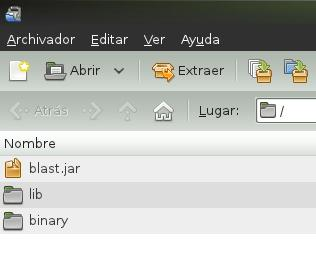
\includegraphics[width=60mm]{./Sections/3_Running_Apps/Figures/example_package.jpeg}
    \caption{An example package. \label{fig:example_package}}
\end{figure}



\subsection{Running the application}
\label{subsec:running_apps}

To run the application on the SDK VM, the path of the application jar must be added to {\bf CLASSPATH} system variable:

\begin{lstlisting}[language=bash]
user@bsccompss:~$ cp ~/workspace/simple/package/Simple.tar.gz   /home/user/
user@bsccompss:~$ tar xzf Simple.tar.gz
user@bsccompss:~$ export CLASSPATH=$CLASSPATH:/home/user/simple.jar
\end{lstlisting}

Once the execution environment is ready, the application can be launched through the following command:

\begin{lstlisting}[language=bash]
user@bsccompss:~$ runcompss simple.Simple <initial_number>
\end{lstlisting}

\begin{figure}[h!]
  \centering
    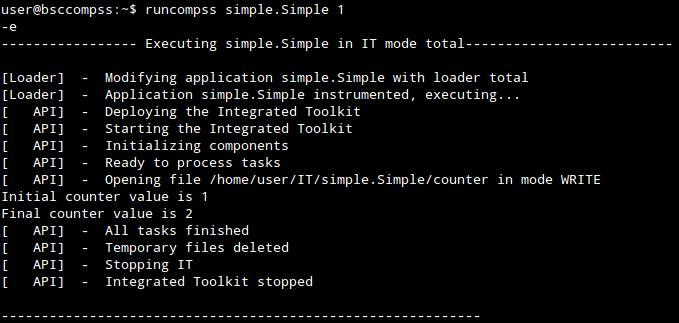
\includegraphics[width=0.95\textwidth]{./Sections/3_Running_Apps/Figures/compss_execution.jpeg}
    \caption{Execution of a COMPSs application. \label{fig:compss_execution}}
\end{figure}
\vspace{-0.4cm}


\subsection{Logging the execution}
The {\bf it.log} file, that can be found generally in {\bf \$HOME/it.log} ({\bf /home/user/it.log, in case of SDK VM}). It shows information on the execution of the application including file transfers and job submission details.

\begin{lstlisting}[language=bash]
user@bsccompss:~$ tail -f it.log
\end{lstlisting}

On the other hand, the {\bf resources.log} file, that can be found in {\bf \$HOME/resources.log}. It shows information about the available resources such as: number of processors of each resource (slots), information about running or pending tasks in the resource queue as depicted in the following picture:

\begin{figure}[h!]
  \centering
    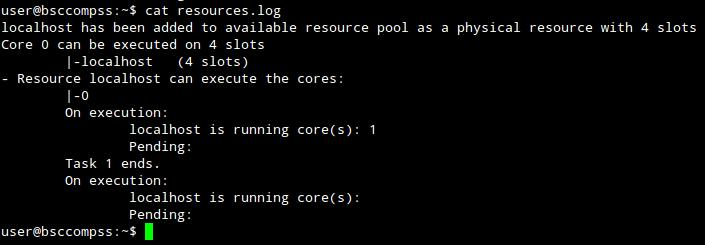
\includegraphics[width=0.95\textwidth]{./Sections/3_Running_Apps/Figures/available_resources.jpeg}
    \caption{Information on the available resources. \label{fig:available_resources}}
\end{figure}


\subsection{Execution results}
After the execution, COMPSs stores the files corresponding to the {\bf stdout} and {\bf stderr} of each task in the {\bf /home/user/IT/APPNAME/} directory.

\begin{figure}[h!]
  \centering
    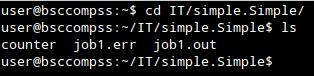
\includegraphics[width=0.6\textwidth]{./Sections/3_Running_Apps/Figures/task_log1.jpeg}
    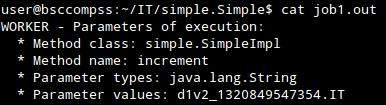
\includegraphics[width=0.6\textwidth]{./Sections/3_Running_Apps/Figures/task_log2.jpeg}
    \caption{The log of each task can be retrieved at the end of the execution. \label{fig:task_logs}}
\end{figure}

The results of an execution will be stored in the {\bf /home/user/IT/simple.Simple/} directory in the example application.


\subsection{Exploring the final execution graph}
At the end of the execution a dependency graph can be generated representing the order of execution of each type of task and their dependencies.

\begin{lstlisting}[language=bash]
user@bsccompss:~$ gengraph graph.dot
\end{lstlisting}

\begin{figure}[h!]
  \centering
    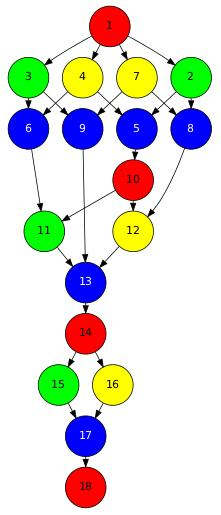
\includegraphics[width=0.3\textwidth]{./Sections/3_Running_Apps/Figures/dependency_graph.jpeg}
    \caption{The dependency graph of the SparseLU application. \label{fig:dependency_graph}}
\end{figure}

\subsection{COMPSs monitoring system}
The COMPSs runtime exposes a Web Service with a graphical interface that can be used to monitor the progress of running applications. In order to see it, a specific URL must be used in a web browser:

\begin{lstlisting}[language=bash]
http://localhost:8080/compss-monitor
\end{lstlisting}

As it can be seen in Figure \ref{fig:monitoring_interface}, the interface gives details about the execution graph (it can be seen how the data dependency graph is built and consumed at real time, and the status of the tasks), the resource usage information, the number of tasks, and the execution time per task.

\begin{figure}[thb!]
  \centering
    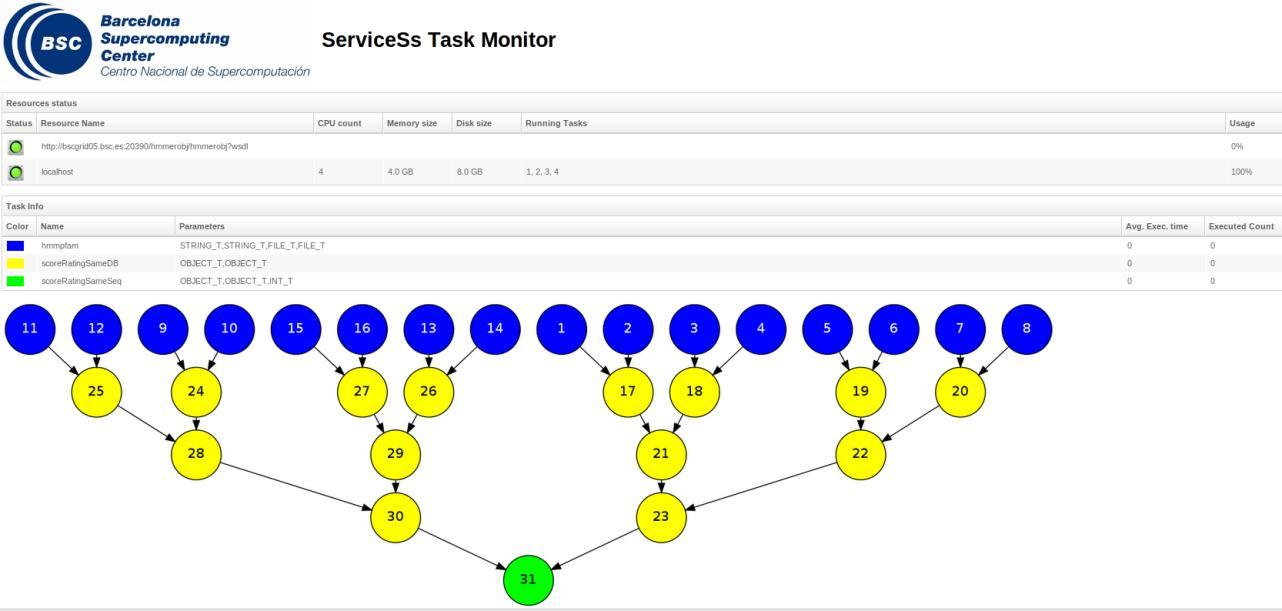
\includegraphics[width=0.9\textwidth]{./Sections/3_Running_Apps/Figures/compss_monitoring.jpeg}
    \caption{COMPSs monitoring interface example. \label{fig:monitoring_interface}}
\end{figure}
           
  \section{Sample applications}
\label{sec:SampleApps}

The examples in this section consider the execution in a cloud platform where the VMs mount a common storage on {\bf /sharedDisk} directory. This is useful in the case of applications that require working with big files, allowing to transfer data only once, at the beginning of the execution, and to enable the application to access the data directly during the rest of the execution.

The Blast sample workflows available in the development environment and explained in the next section takes advantage of this functionality.

The development environment provides some sample COMPSs applications that can be found in {\bf /home/user/workspace/} directory. The following section describes in detail the development of each of them.

\subsection{Matrix multiplication}
Matrix Multiplication (Matmul) is a pure Java application that multiplies two matrices in a direct way. The application creates 2 matrices of N x N size initialized with values, and multiply the matrices by blocks of 40 floats (by default).

\begin{figure}[ht!]
  \centering
    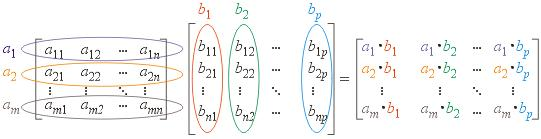
\includegraphics[width=0.8\textwidth]{./Sections/4_Sample_Apps/Figures/matrix.jpeg}
    %\caption{Matrix multiplication. \label{fig:matrix}}
\end{figure}

In this application the multiplication is implemented in the multiplyAccumulative that is thus selected as the task that will be executed remotely. In order to run the application the matrix dimension has to be supplied.

\begin{lstlisting}[language=bash]
user@bsccompss:~$ cp ~/workspace/matmul/package/Matmul.tar.gz /home/user/
user@bsccompss:~$ tar xzf Matmul.tar.gz
user@bsccompss:~$ export CLASSPATH=$CLASSPATH:/home/user/matmul.jar
\end{lstlisting}

The command line to execute the application:

\begin{lstlisting}[language=bash]
user@bsccompss:~$ runcompss matmul.Matmul <matrix_dim>
\end{lstlisting}


\subsection{Sparse LU decomposition}
SparseLU multiplies two matrices using the factorization method of LU decomposition, which factorizes a matrix as a product of a lower triangular matrix and an upper one.

\begin{figure}[ht!]
  \centering
    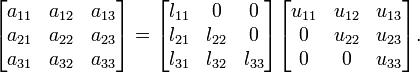
\includegraphics[width=0.6\textwidth]{./Sections/4_Sample_Apps/Figures/SparseLU.jpeg}
    %\caption{Sparse LU decomposition\label{fig:SparseLO}}
\end{figure}

The matrix is divided into N x N blocks on where 4 types of operations will be applied modifying the blocks: {\bf lu0}, {\bf fwd}, {\bf bdiv} and {\bf bmod}. These four operations are implemented in four methods that are selecetd as the tasks that will be executed remotely. In order to run the application the matrix dimension has to be provided.

\begin{lstlisting}[language=bash]
user@bsccompss:~$ cp ~/workspace/sparselu/package/SparseLU.tar.gz /home/user/
user@bsccompss:~$ tar xzf SparseLU.tar.gz
user@bsccompss:~$ export CLASSPATH=$CLASSPATH:/home/user/sparselu.jar
\end{lstlisting}

The command line to execute the application:

\begin{lstlisting}[language=bash]
user@bsccompss:~$ runcompss sparselu.SparseLU <matrix_dim>
\end{lstlisting}

\subsection{BLAST Workflow}
BLAST is a widely-used bioinformatics tool for comparing primary biological sequence information, such as the amino-acid sequences of different proteins or the nucleotides of DNA sequences with sequence databases, identifying sequences that resemble the query sequence above a certain threshold. The work performed by the COMPSs Blast workflow is computationally intensive and embarrassingly parallel.

\begin{figure}[ht!]
  \centering
    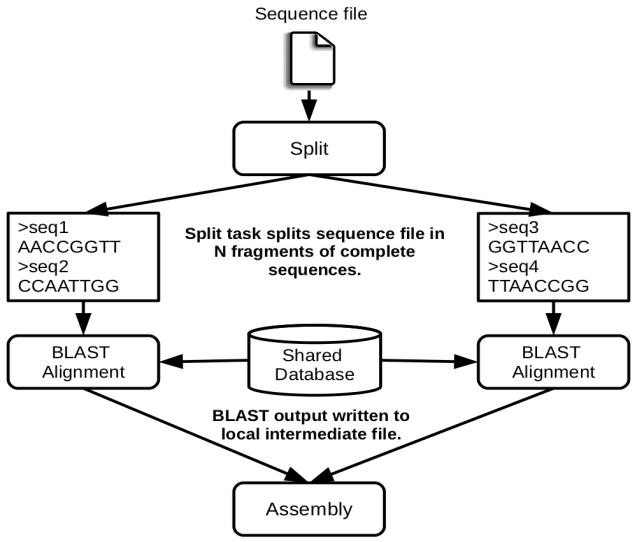
\includegraphics[width=0.7\textwidth]{./Sections/4_Sample_Apps/Figures/blast_workflow.jpeg}
    \caption{The COMPSs Blast workflow. \label{fig:BLAST_workflow}}
\end{figure}

The workflow describes the three blocks of the workflow implemented in the {\bf Split}, {\bf Align} and {\bf Assembly} methods. The second one is the only method that is chosen to be executed remotely, so it is the unique method defined in the interface file. The {\bf Split} method chops the query sequences file in N fragments, {\bf Align} compares each sequence fragment against the database by means of the Blast binary, and {\bf Assembly} combines all intermediate files into a single result file.

This application uses a database that will be on the shared disk space avoiding transferring the entire database (which can be large) between the virtual machines.

\begin{lstlisting}[language=bash]
user@bsccompss:~$ cp ~/workspace/blast/package/Blast.tar.gz      /home/user/
user@bsccompss:~$ tar xzf Blast.tar.gz
user@bsccompss:~$ export CLASSPATH=$CLASSPATH:/home/user/blast.jar
\end{lstlisting}

The command line to execute the workflow:

\begin{lstlisting}[language=bash]
user@bsccompss:~$ runcompss blast.Blast <debug> <bin_location>
                                        <database_file> 
                                        <sequences_file>
                                        <frag_number> <tmpdir>
                                        <output_file>
\end{lstlisting}

Where:

\begin{itemize}
 \item {\bf debug}: The debug flag of the application (true or false).
 \item {\bf bin\_location}: Path of the Blast binary.
 \item {\bf database\_file}: Path of database file; the shared disk {\bf /sharedDisk/} is suggested to avoid big data transfers.
 \item {\bf sequences\_file}: Path of sequences file.
 \item {\bf frag\_number}: Number of fragments of the original sequence file, this number determines the number of parallel Align tasks.
 \item {\bf tmpdir}: Temporary directory ({\bf /home/user/tmp/}).
 \item {\bf output\_file}: Path of the result file.
\end{itemize}
 
Example:

\begin{lstlisting}[language=bash]
user@bsccompss:~$ runcompss blast.Blast true

/home/user/workspace/blast/binary/blastall
/sharedDisk/Blast/databases/swissprot/swissprot
/sharedDisk/Blast/sequences/sargasso_test.fasta 4 /tmp/
/home/user/out.txt
\end{lstlisting}
           
  \section{COMPSs Configuration}
\label{sec:COMPSsConfiguration}

COMPSs SDK VM is a preconfigured light 64-bit Xubuntu distribution providing the necessary set of tools to develop COMPSs applications. The development environment includes an {\bf Eclipse IDE}, the {\bf COMPSs framework} and a set of {\bf sample applications} in order to ease the comprehension of the programing model in a more straightforward way.

The COMPSs framework is installed in {\it /opt/COMPSs/}.

For the development of new projects in Eclipse please remember to add the reference to the COMPSs runtime adding {\it /opt/COMPSs/Runtime/rt/compss-rt.jar} as referenced library. 

Please note that in case of changing the number of available cores in the physical SDK machine, this should be reflected in the COMPSs configurations files, {\bf resources.xml} ({\it LimitOfTasks}) and {\bf project.xml} ({\it CPUCount}), as indicated in the picture.

{\bf project.xml}

\begin{lstlisting}[language=xml]
user@bsccompss:~$ cat /opt/COMPSs/Runtime/xml/projects/project.xml
<?xml version="1.0" encoding="UTF-8"?>
<Project>
    <!--Description for any physical node-->
    <Worker Name="localhost">
        <InstallDir>/IT_worker/</InstallDir>
        <WorkingDir>/home/user/</WorkingDir>
        <User>user</User>
        <LimitOfTasks>2</LimitOfTasks>
    </Worker>
</Project>
\end{lstlisting}

{\bf resources.xml}

\begin{lstlisting}[language=xml]
user@bsccompss:~$ cat /opt/COMPSs/Runtime/xml/resources/resources.xml
<?xml version="1.0" encoding="UTF-8"?>
<ResourceList>
    <!--Description for any physical node-->
    <Resource Name=“localhost">
        <Capabilities>
            <Host>
                <TaskCount>0</TaskCount>
                <Queue>short</Queue>
                <Queue/>
            </Host>
            <Processor>
                <Architecture>IA32</Architecture>
                <Speed>3.0</Speed>
                <CPUCount>2</CPUCount>
            </Processor>
            <OS>
                <OSType>Linux</OSType>
                <MaxProcessesPerUser>32</MaxProcessesPerUser>
            </OS>
            <StorageElement>
                <Size>30</Size>
            </StorageElement>
            <Memory>
                <PhysicalSize>2</PhysicalSize>
                <VirtualSize>8</VirtualSize>
            </Memory>
                <ApplicationSoftware>
                <Software>Java</Software>
            </ApplicationSoftware>
            <Service/>
            <VO/>
            <Cluster/>
            <FileSystem/>
            <NetworkAdaptor/>
            <JobPolicy/>
            <AccessControlPolicy/>
        </Capabilities>
        <Requirements/>
    </Resource>
</ResourceList>
\end{lstlisting}
     
In order to use external resources to execute the applications, the following steps have to be followed:

\begin{enumerate}
 \item Install the COMPSs framework on the new resources following the installation manual available at \url{http://www.bsc.es/compss}.
 \item Edit the {\bf resources.xml} and {\bf project.xml} files in the master machine (the SDK VM) in order to be aware of the new resources (Section \ref{sec:SampleApps}).
 \item Create/set the WorkingDir in the path specified in {\bf project.xml}.
 \item Set SSH passwordless access to the rest of the remote resources.
 \item In case of cloud resources the application will be deployed automatically, and this, should be set up on COMPSs configuration files. In case of static resources, deploy the  application manually on the new ones (see section \ref{subsec:compiling_and_packaging_apps} and \ref{subsec:running_apps}).
\end{enumerate}

\subsection{Cluster configuration (static resources)}

On the following lines, we provide examples about configuration files for Grid and Cluster environments, which can serve as a reference. They can also be compared to the examples previously provided to see the differences in such scenarios.

\subsubsection{Resources}

\begin{lstlisting}[language=xml]
<?xml version="1.0" encoding="UTF-8"?>
<ResourceList>
    <!--Description for any physical node-->
    
    <Resource Name="172.20.200.18">
        <Capabilities>
            <Host>
                <TaskCount>0</TaskCount>
                <Queue>short</Queue>
                <Queue/>
            </Host>
            <Processor>
                <Architecture>IA32</Architecture>
                <Speed>3.0</Speed>
                <CPUCount>1</CPUCount>
            </Processor>
            <OS>
                <OSType>Linux</OSType>
                <MaxProcessesPerUser>32</MaxProcessesPerUser>
            </OS>
            <StorageElement>
                <Size>30</Size>
            </StorageElement>
            ...
            <Memory>
                <PhysicalSize>1</PhysicalSize>
                <VirtualSize>8</VirtualSize>
            </Memory>
            <ApplicationSoftware>
                <Software>Java</Software>
            </ApplicationSoftware>
            <Service/>
            <VO/>
            <Cluster/>
            <FileSystem/>
            <NetworkAdaptor/>
            <JobPolicy/>
            <AccessControlPolicy/>
        </Capabilities>
        <Requirements/>
    </Resource>
    
    <Resource Name="172.20.200.19">
    ...
    </Resource>
    
<ResourceList>
\end{lstlisting}

\subsubsection{Project}
\begin{lstlisting}[language=xml]
<?xml version="1.0" encoding="UTF-8"?>
<Project>
  <!--Description for any physical node-->
    
  <Worker Name="172.20.200.18">
    <InstallDir>/opt/COMPSs/Runtime/scripts/system/</InstallDir>
    <WorkingDir>/tmp/</WorkingDir>
    <User>user</User>
    <LimitOfTasks>1</LimitOfTasks>
  </Worker>
    
  <Worker Name="172.20.200.19">
  ...
  </Worker>
    
  ...
</Project>
\end{lstlisting}

\subsection{Shared Disks configuration}
Configuring shared disks on the runtime configuration might reduce the amount of data transfers improving the application performance. To indicate a shared disk hosted in the master node, the resources list in the resources.xml file must include a disk tag describing the disk and the mount point. The following example of resources.xml states that in the master node there is a shared disk labelled {\it sharedDisk0} mounted on the {\it /home/user} directory.

\begin{lstlisting}[language=xml]
<?xml version="1.0" encoding="UTF-8"?>
<ResourceList>
    <Disk Name="sharedDisk0">
        <MountPoint>/home/user</MountPoint>
    </Disk>
<ResourceList>
\end{lstlisting}

On the other side, also worker nodes description in the {\bf resource.xml} file should declare the shared disks mounted on them to avoid data transfers as done for {\it sharedDisk0} in the following example. Though, the example only contains the definition of a single shared disk, the Disks tag can have multiple disk child nodes.

\begin{lstlisting}[language=xml]
<Resource Name="172.20.200.18">
    <Capabilities>
    ...
    </Capabilities>
    <Requirements/>
    <Disks>
        <Disk Name="sharedDisk0">
            <MountPoint>/home/user</MountPoint>
        </Disk>
    </Disks>
</Resource>
\end{lstlisting}

\subsection{Cloud Provider configuration (dynamic resources)}

The COMPSs runtime communicates with the Cloud by means of Cloud connectors. Each connector implements the interaction of the runtime with a given Cloud provider, more precisely by supporting four basic operations: ask for the price of a certain VM in the provider, get the time needed to create a VM, create a new VM and terminate a VM.

Connectors abstract the runtime from the particular API of each provider; furthermore, this design facilitates the addition of new connectors for other providers.

The next subsections describe the basic configuration options for Cloud provider connectors and provide a description of each of the connectors currently available.

Connectors can be configured by providing some information in the {\bf resources.xml} and {\bf project.xml} files. These files are located at $<COMPSs\_INSTALL\_DIR>/xml/projects$ and $<COMPSs\_INSTALL\_DIR>/xml/resources$. The example folders in these directories contain some respective examples for different backends.

\subsubsection{Resources}
The resources.xml file can contain one or more tags {\bf $<CloudProvider>$} that encompass the information about a particular Cloud provider, associated to a given connector. The tag must have an attribute {\bf name} to uniquely identify the provider. Table \ref{tab:conf_resources_xml} summarizes the information to be specified by the user inside this tag.


\begin{longtable}{| p{0.50\textwidth} | p{0.50\textwidth} |}
\hline
Server			&		Endpoint of the provider’s server	\\
\hline
Connector		&		Class that implements the connector	\\
\hline
\textbf{
ImageList
\begin{itemize}
 \item Image
 \begin{itemize}
  \item Architecture
  \item OSType
  \item ApplicationSoftware
  \begin{itemize}
   \item Software
  \end{itemize}
  \item SharedDisks
  \begin{itemize}
   \item Disk
  \end{itemize}
 \end{itemize}
\end{itemize}
}
&
Multiple entries of VM templates
\begin{itemize}
 \item VM image
 \begin{itemize}
  \item Architeture of the VM image
  \item Operative System installed in the VM image
  \item Multiple entries of software installed in the VM image
  \begin{itemize}
   \item Software installed in the VM image
  \end{itemize}
  \item Multiple entries of shared disks mounted in the VM image
  \begin{itemize}
   \item Disk description
  \end{itemize}
 \end{itemize}
\end{itemize}
\\
\hline
\textbf{
InstanceTypes
\begin{itemize}
 \item Resource
 \begin{itemize}
  \item Capabilities
  \begin{itemize}
   \item Processor
   \item StorageElement
   \item Memory
  \end{itemize}
 \end{itemize}
\end{itemize}
}
& 
Multiple entries of resource templates
\begin{itemize}
 \item Instance type offered by the provider
 \begin{itemize}
  \item Hardware details of instance type
  \begin{itemize}
   \item Architecture and number of available cores
   \item Size in GB of the storage
   \item PhysicalSize, in GB of the available RAM
  \end{itemize}
 \end{itemize}
\end{itemize}
\\
\hline
\caption{Configuration of resources.xml file, tag $<CloudProvider>$}
\label{tab:conf_resources_xml}
\end{longtable}


\subsubsection{Project}
The project.xml complements the information about Cloud providers specified in the resources.xml file. This file can contain a {\bf $<Cloud>$} tag where to specify a list of providers, each with a {\bf $<Provider>$} tag, whose {\bf name} attribute must match one of the providers in the {\it resources.xml} file. Thus, the {\it project.xml} file must contain a subset of the providers specified in the resources.xml file. Table \ref{tab:conf_project_xml_cloud} summarizes the information to be specified by the user in the {\bf $<Provider>$} tags of the {\it project.xml} file.

\begin{table}[h]
\footnotesize
\begin{center}
\begin{tabularx}{\textwidth}{|>{\setlength\hsize{1.0\hsize}\setlength\linewidth{\hsize}}X|>{\setlength\hsize{1.0\hsize}\setlength\linewidth{\hsize}}X|}
\hline
InitialVMs	&	Number of VM to be created at the beginning of the application	\\
\hline
minVMCount	&	Minimum number of VMs available in the computation	\\
\hline
maxVMCount	&	Maximum number of VMs available in the computation	\\
\hline
Provider 	&	Multiple entries of Cloud providers	\\
\hline
\end{tabularx}
\caption{Configuration of project.xml file, tag $<Cloud>$\label{tab:conf_project_xml_cloud}}
\end{center}
\end{table}


\begin{longtable}{| p{0.43\textwidth} | p{0.57\textwidth} |}
\hline
LimitOfVMs	&	Maximum number of VMs allowed by the provider	\\
\hline
Property
\begin{itemize}
 \item Name
 \item Value
\end{itemize}
&
Multiple entries of provider-specific properties
\begin{itemize}
 \item Name of the property
 \item Value of the property
\end{itemize}
\\
\hline
ImageList
\begin{itemize}
 \item Image
 \begin{itemize}
  \item InstallDir
  \item WorkingDir
  \item User
  \item Package
  \begin{itemize}
   \item Source
   \item Target
   \item InstalledSoftware
  \end{itemize}
 \end{itemize}
\end{itemize}
& 
Multiple entries of VM images available at the provider
\begin{itemize}
 \item VM image
  \begin{itemize}
   \item Path of the COMPSs worker scripts in the image
   \item COMPSs working directory in the deployed instances
   \item Account username
   \item Multiple entries of local packages that have to be deployed in new instances
   \begin{itemize}
    \item Local path of the package
    \item Path where to deploy the package in the new instance
    \item List of software included in the package
  \end{itemize}
 \end{itemize}
\end{itemize}
\\
\hline
InstanceTypes
\begin{itemize}
 \item Resource
\end{itemize}
& 
List of resource types that are available in the provider
\begin{itemize}
 \item Resource description
\end{itemize}

\\
\hline
\caption{Configuration of project.xml file, tag $<Provider>$}
\label{tab:conf_project_xml_provider}
\end{longtable}


\subsection{Connectors}
\subsubsection{Amazon EC2}

The COMPSs runtime features a connector to interact with the Amazon Elastic Compute Cloud (EC2).

Amazon EC2 offers a well-defined pricing system for VM rental. A total of 8 pricing zones are established, corresponding to 8 different locations of Amazon datacenters around the globe. Besides, inside each zone, several per-hour prices exist for VM instances with different capabilities. The EC2 connector stores the prices of standard on-demand VM instance types (t1.micro, m1.small, m1.medium, m1.large and m1.xlarge) for each zone. Spot instances are not currently supported by the connector.

When the COMPSs runtime chooses to create a VM in the Amazon public Cloud, the EC2 connector receives the information about the requested characteristics of the new VM, namely the number of cores, memory, disk and architecture (32/64 bits). According to that information, the connector tries to find the VM instance type in Amazon that better matches those characteristics and then requests the creation of a new VM instance of that type.

Once an EC2 VM is created, a whole hour slot is paid in advance; for that reason, the connector keeps the VM alive at least during such period, saving it for later use if necessary. When the task load decreases and a VM is no longer used, the connector puts it aside if the hour slot has not expired yet, instead of terminating it. After that, if the task load increases again and the EC2 connector requests a VM, first the set of saved VMs is examined in order to find a VM that is compatible with the requested characteristics. If one is found, the VM is reused and becomes eligible again for the execution of tasks; hence, the cost and time to create a new VM are not paid. A VM is only destroyed when the end of its hour slot is approaching and it is still in saved state.

Table \ref{tab:conf_project_xml_provider} summarizes the provider-specific properties that must be defined in the project.xml file for the Amazon EC2 connector.

\begin{longtable}{| p{0.3\textwidth} | p{0.7\textwidth} |}
\hline
{\bf Placement }    &   Location of the amazon datacentre to use \\
\hline
Access Key Id       &   Identifier of the access key of the Amazon EC2 account \\
\hline
Secret Key Id       &   Identifier of the secret key of the Amazon EC2 account \\
\hline
Key host location   &   Path to the SSH key in the local host, used to connect to the VMs \\
\hline
KeyPair name        &   Name of the key pair to use \\
\hline
SecurityGroup name  &   Name of the security group to use \\
\hline
\caption{Properties of the Amazon EC2 connector.}
\label{tab:ec2_connector_properties}
\end{longtable}

\vspace{-1.0cm}

\subsubsection{rOCCI Connector}
In order to execute a COMPSs application in the cloud, the rOCCI connector has to be configured properly. The connector uses the rOCCI binary client\footnote{\url{https://appdb.egi.eu/store/software/rocci.cli}} (version newer or equal than 4.2.5) which has to be installed in the node where the COMPSs main application is executed.

This connector needs additional files providing details about the resource templates available on each provider. This file is located under $<COMPSs\_INSTALL\_DIR>/xml/templates$ path. Additionally, the user must define the virtual images flavour and instance types offered by each provider; thus, when the runtime asks for the creation of a VM, the connector selects the appropriate image and resource template according to the requirements (in terms of CPU, memory, disk, etc) by invoking the rOCCI client through Mixins (heritable classes that override and extend the base templates).

Table \ref{tab:rOCCI_extensions} contains the rOCCI specific properties that must be defined in the project.xml file.

\begin{longtable}{| p{0.25\textwidth} | p{0.75\textwidth} |}
\hline
{\bf Provider }    &  \\
\hline
ca-path     &   Path to CA certificates directory \\
\hline
user-cred   &   Path of the VOMS proxy \\
\hline
auth        &   Authentication method, x509 only supported \\
\hline
owner & \multirow{2}{*}{Optional. Used by the VENUS-C Job Manager (PMES)} \\
\cline{1-1}
jobname &  \\
\hline
\caption{rOCCI extensions in the project.xml file.}
\label{tab:rOCCI_extensions}
\end{longtable}

\vspace{-0.75cm}

\begin{longtable}{| p{0.25\textwidth} | p{0.75\textwidth} |}
\hline
{\bf Instance} & Multiple entries of resource templates. \\
\hline
Type   &    Name of the resource template. It has to be the same name than in the previous files \\
\hline
CPU    &    Number of cores \\
\hline
Memory &    Size in GB of the available RAM \\
\hline
Disk   &    Size in GB of the storage \\
\hline
Price  &    Cost per hour of the instance \\
\hline
\caption{Configuration of the $<provider>.xml$ templates file.}
\label{tab:rOCCI_configuration}
\end{longtable}


           
  \section{Bindings}
\label{sec:Bindings}

In addition to Java, COMPSs supports the execution of applications written in other languages by 
means of bindings. A binding manages the interaction of the not-Java application with the COMPSs 
Java runtime, providing the necessary language translation.

The next subsections describe the language bindings provided by COMPSs.

\subsection{C/C++}

COMPSs provides a binding for C and C++ applications. The new C++ version in the current release 
comes with support for objects as task parameters and the use of class methods as tasks.

\subsubsection{Programming Model}

\paragraph{Task Selection}
As in Java language the user must write the task selection like an ``interface''. In this case 
the interface file has the same name as the main application file plus the suffix ``idl'', 
i.e. Matmul.idl, where the main file is called Matmul.cc.

\begin{lstlisting}[language=C++]
interface Matmul
{
      // C functions
      void initMatrix(inout Matrix matrix,
                      in int mSize,
                      in int nSize,
                      in double val);
                      
      void multiplyBlocks(inout Block block1,
                          inout Block block2,
                          inout Block block3);
                          
      // C++ class methods
      void Block::multiply(in Block block1,
                           in Block block2);
                           
      static Matrix Matrix::init(in int mSize,
                                 in int bSize,
                                 in double val);
};
\end{lstlisting}

The syntax of the interface file is shown in the previous code. Tasks can be declared as classic 
C function prototypes, this allow to keep the compatibility with standard C applications. 
In the example, initMatrix and multiplyBlocks are functions declared using its prototype, 
like in a C header file, but this code is C++ as they have objects as parameters (objects of 
type Matrix, or Block).

A class method can be also a task, and it is declared using its signature. In the example, 
Block::multiply and Matrix::init are class methods. In this example, C functions encapsulates 
object method calls, as we will see later.

The grammar for the interface file is as follows:

\begin{lstlisting}[language=bash]
["static"] return-type task-name ( parameter {, parameter }* );

return-type = "void" | type

ask-name = <qualified name of the function or method>

parameter = direction type parameter-name

direction = "in" | "out" | "inout"

type = "char" | "string" | "int" | "short" | "long"
    | "float" | "double" | "boolean" | "File" | class-name

class-name = <qualified name of the class>
\end{lstlisting}

       
\paragraph{Value and Object return}
Notice that returning a value or an object is now supported, this means a ``void'' value, a value 
of a primitive type (an int, long, float, etc.), or an object of a class, can be returned from a 
function or method.

{\bf IMPORTANT:}

In C/C++ the default policy is to make a copy of the value or object when it is returned [A = foo();], 
and this copy (A) is a new position in memory whom reference or address is not possible to know before 
the return statement.

As the binding can’t know such reference before leaving the task execution (foo) it must do a 
synchronization before the return statement for the correct value to be copied when returning. 
This is called an explicit synchronization.

Alternatively, the return of a value or an object can be done also by mean of an out or inout parameter, 
and no explicit synchronization is needed because the reference is passed to the binding in this case 
using de \& operator [foo(\&A);].

\paragraph{Main Program}
The main program is a sequential code written in C++ that launches tasks to be executed in parallel 
and may have several data-synchronization points or none.

\begin{lstlisting}[language=C++]
#define %*{\bf DEBUG\_BINDING }*)
#include %*{\bf "Matmul.h" }*)
#include "Matrix.h"
#include ""Block.h"
int N; //MSIZE
int M; //BSIZE
double val;
int main(int argc, char **argv)
{
      Matrix A;
      Matrix B;
      Matrix C;

       N = atoi(argv[1]);
       M = atoi(argv[2]);
      val = atof(argv[3]);

      %*{\bf compss\_on(); }*)

      A = Matrix::init(N,M,val);

      initMatrix(&B,N,M,val);
      initMatrix(&C,N,M,0.0);

      cout << "Waiting for initialization...\n";

      %*{\bf compss\_wait\_on(B); }*)
      %*{\bf compss\_wait\_on(C); }*)

      cout << "Initialization ends...\n";
 
      C.multiply(A, B);

      %*{\bf compss\_off(); }*)
      return 0;
}
\end{lstlisting}

The main points when programming the main code are:
\begin{enumerate}
 \item The directive {\bf DEBUG\_BINDING} can be defined if we need debug information from the binding.
 \item A header file with the same name as the main file must be included, in this case {\bf Matmul.h}. 
       This header file is automatically generated by the binding and it contains other includes and 
       certain type-definitions that are needed.
 \item A call to the {\bf compss\_on} binding function to turn on the COMPSs runtime.
 \item As in C language, when passing and out or inout parameter, the memory address should be passed 
       in order the parameter can be modified. For that, in a task-function call, we use the ``{\bf \&}'' 
       operator before the parameter name.
 \item Synchronization on a parameter can be done calling the {\bf compss\_wait\_on} binding function. 
       The argument of this function must be the variable or object we want to synchronize.
 \item There is an {\bf implicit synchronization} in the init method of Matrix. It is not possible to 
       know the address of ``A'' before exiting the method call and due to this it is necessary to synchronize 
       before for the copy of the returned value into ``A'' for it to be correct.
 \item A call to the {\bf compss\_off} binding function to turn off the COMPSs runtime.
\end{enumerate}


\paragraph{Functions file}
The function file is where the programmer writes the implementation of the tasks in a C or C++ function style. 
Its name must be the same as the main file followed by the suffix ``-functions''. In our case Matmul-functions.cc.

\begin{lstlisting}[language=C++]
#include "Matmul.h"
#include "Matrix.h"
#include "Block.h"

void initMatrix(Matrix *matrix,int mSize,int nSize,double val){
     *matrix = Matrix::init(mSize, nSize, val);
}

void multiplyBlocks(Block *block1,Block *block2,Block *block3){
     block1->multiply(*block2, *block3);
}
\end{lstlisting}

There is no special consideration when writing the functions (or tasks), only to include the Matmul.h header file is needed.

In the previous code, class methods have been encapsulated inside a function. 
This is useful when the class method returns an object or a value and we want to avoid the explicit 
synchronization when returning from the method that we have mentioned before.

\paragraph{Other Source Files}
The user application for sure will have other source files than the main-file and the functions-file 
seen in the previous sections. This other files must be placed under the directory ``{\bf src}''.

In this directory the programmer must provide a {\bf Makefile} that compiles such source files in the proper way. 
When the binding compiles the whole application it will enter into the src directory and executes the Makefile.

The previous code shows an example of a Makefile. 
It generates two libraries, one for the master application and another for the worker application. 
The directive COMPSS\_MASTER or COMPSS\_WORKER must be used in order to compile the source files for each type of library. 
Both libraries will be copied into the lib directory where the binding will look for them when generating the master and worker applications.

\paragraph{Class Serialization}
As known, the C++ classes can be written in separated files, a header file for the declaration and a source file for the implementation.

Here we show the class Block. The important thing here is that the class must provide the method for the object serialization. 
This serialization is done using the ``{\bf boost}'' library. The ``{\bf serialize}'' method is implemented inline in the header file.

\begin{lstlisting}[language=C++]
#ifndef BLOCK_H
#define BLOCK_H

#include    <vector>
#include    <boost/archive/text_iarchive.hpp>
#include    <boost/archive/text_oarchive.hpp>
#include    <boost/serialization/serialization.hpp>
#include    <boost/serialization/access.hpp>
#include    <boost/serialization/vector.hpp>

using namespace std;
using namespace boost;
using namespace serialization;

class Block {
public:
    Block(){};

    Block(int bSize);
       
    static Block *init(int bSize, double initVal);
        
    void multiply(Block block1, Block block2);
        
    void print();

private:
    int M;
    std::vector< std::vector< double > > data;
        
    %*{\bf friend class::serialization::access; }*)
    %*{\bf template$<$class Archive$>$ }*)
    %*{\bf void serialize(Archive \& ar, const unsigned int version) \{ }*)
        %*{\bf ar \& M; }*)
        %*{\bf ar \& data; }*)
    %*{\bf \} }*)
};

#endif
\end{lstlisting}

For more information about serialization using ``boost'' visit the related documentation at \url{www.boost.org}.


\paragraph{Method – Task}

A task can be a C++ class method. A method can return a value, modify the “this” object, or modify a parameter.

If the method has a return value there will be an implicit synchronization before exit the method, 
but for the “this” object and parameters the synchronization can be done later after the method has finished.

This is due to the ``this'' object and parameters can be accessed inside the method and outside, but for the 
variable where the returned value is copied to, it can’t be known inside the method.

\begin{lstlisting}[language=C++]
#include "Block.h"

Block::Block(int bSize) {
       M = bSize;
       data.resize(M);
       for (int i=0; i<M; i++) {
              data[i].resize(M);
       }
}

Block *Block::init(int bSize, double initVal) {
       Block *block = new Block(bSize);
       for (int i=0; i<bSize; i++) {
              for (int j=0; j<bSize; j++) {
                     block->data[i][j] = initVal;
              }
       }
       return block;
}

#ifdef COMPSS_WORKER

void Block::multiply(Block block1, Block block2) {
       for (int i=0; i<M; i++) {
              for (int j=0; j<M; j++) {
                     for (int k=0; k<M; k++) {
                            data[i][j] += block1.data[i][k] * block2.data[k][j];
                     }
              }
       }
       this->print();
}

#endif

void Block::print() {
       for (int i=0; i<M; i++) {
              for (int j=0; j<M; j++) {
                     cout << data[i][j] << " ";
              }
              cout << "\r\n";
       }
}
\end{lstlisting}

\paragraph{XML configuration files}
The project.xml and the resources.xml files as in Java language must be provided to the COMPSs runtime. 
This files must be found in the same directory as the main file.

Here is the project.xml file for the Test application.

\begin{lstlisting}[language=xml] 
<?xml version="1.0" encoding="UTF-8"?>
<Project>
  <Worker Name="localhost">
    <InstallDir>/opt/COMPSs/Runtime/scripts/system/</InstallDir>
<WorkingDir>/home/user/matmul_objects/worker/files/</WorkingDir>
    <AppDir>/home/user/matmul_objects/worker/</AppDir>
    <User>user</User>
    <LimitOfTasks>4</LimitOfTasks>
  </Worker>
</Project>
\end{lstlisting}

Here is the resources.xml

\begin{lstlisting}[language=xml] 
<?xml version="1.0" encoding="UTF-8"?>
<ResourceList>
    <Resource Name="localhost">
        <Capabilities>
            <Host>
                <TaskCount>0</TaskCount>
                <Queue>short</Queue>
                <Queue/>
            </Host>
            <Processor>
                <Architecture>IA32</Architecture>
                <Speed>3.0</Speed>
                <CPUCount>4</CPUCount>
            </Processor>
            <OS>
                <OSType>Linux</OSType>
                <MaxProcessesPerUser>32</MaxProcessesPerUser>
            </OS>
            <StorageElement>
                <Size>8</Size>
            </StorageElement>
            <Memory>
                <PhysicalSize>4</PhysicalSize>
                <VirtualSize>8</VirtualSize>
            </Memory>
            <ApplicationSoftware>
                <Software>Java</Software>
            </ApplicationSoftware>
            <Service/>
            <VO/>
            <Cluster/>
            <FileSystem/>
            <NetworkAdaptor/>
            <JobPolicy/>
            <AccessControlPolicy/>
        </Capabilities>
        <Requirements/>
    </Resource>
</ResourceList>
\end{lstlisting}

\subsubsection{Application Compilation}
In order to compile the user application against the binding libraries in a proper way a script is 
accessible in the system path after the binding installation.

In the same directory where the main file resides, just execute the command ``{\bf buildapp}'' and 
pass the name of the application as argument to this script, in this case ``Matmul''.

\begin{lstlisting}[language=bash]
user@localhost:~/matmul_objects$ buildapp Matmul

Building application...

g++ -DCOMPSS_MASTER -g -I. -I/opt/COMPSs/Runtime/bindings/c/include -I/opt/COMPSs/Runtime/bindings/bindings-common/include -c Block.cc Matrix.cc ar rvs libmaster.a Block.o Matrix.o

g++ -DCOMPSS_WORKER -g -I. -I/opt/COMPSs/Runtime/bindings/c/include -I/opt/COMPSs/Runtime/bindings/bindings-common/include -c Block.cc Matrix.cc ar rvs libworker.a Block.o Matrix.o

Building all:

Building Master...

g++ -g -O2 -o Matmul Matmul-empty.o Matmul-stubs.o Matmul.o -L../../lib -lmaster -L/usr/lib/jvm/java-6-openjdk-amd64/jre/lib/amd64/server -ljvm -ldl -L/opt/COMPSs/Runtime/bindings/c/../bindings-common/lib -lbindings_common -L/opt/COMPSs/Runtime/bindings/c/lib -lcbindings -lboost_iostreams -lboost_serialization

Building Worker...

g++ -g -O2 -o Matmul-worker Matmul-worker.o Matmul-functions.o -L../../lib -lworker -ldl -lboost_iostreams -lboost_serialization -L/opt/COMPSs/Runtime/bindings/c/lib

Command succesful.
\end{lstlisting}

\emph{[The previous output has been cut for simplicity]}

\subsubsection{Application Environment}
The following environment variables must be defined before executing a COMPSs C/C++ application:
            
\begin{center}
JAVA\_HOME: Java JDK installation directory 

(e.g. /usr/lib/jvm/java-6-openjdk/)
\end{center}


\subsubsection{Application Execution}
After compiling the application, two directories are generated, the master and the worker directories. 
The master directory contains a binary called as the main file, which is the master application, in our 
example is called Matmul. The worker directory contains another binary called as the main file followed 
by the suffix ``-worker'', which is the worker application, in our example is called Matmul-worker.

In order to run the whole application, master and worker applications, use the ``{\bf runcompssext}'' 
script that can be found in the system path after the runtime installation. Here is the example of the 
command execution for the Matmul application.

\begin{lstlisting}[language=bash]
user@localhost:~/runcompssext
         --app=/home/user/matmul_objects/master/Matmul
         --project=/home/user/matmul_objects/project.xml
         --resources=/home/user/matmul_objects/resources.xml
         --lang=c
         --graph=true
         --tracing=false
         --cline_args="3 4 2.0"
\end{lstlisting}

The options of the script are:
\begin{lstlisting}[language=bash]
      --lang=c
      --app=<path>: path to the binary file containing the main program.
      --classpath=<path>: path/s where to search for the application's modules.
      The default value is the current directory.
      --library_path=<path>: path/s where to search for libraries that are not in a standard path.
      The default value is the variable $LD_LIBRARY_PATH.
      --cline_args=<args>: arguments to pass to the application.
      --project=<proj_file>: path of the project XML file.
      --resources=<res_file>: path of the resources XML file.
      --tracing=<true | false>: generate execution traces.
      The default value is false.
\end{lstlisting}

\subsubsection{Matmul Execution Graph}
This is the execution graph for the matmul application in its object version with 3x3 matrices of blocks. 
That means a total of 9 blocks where each block is another 4x4 matrix of doubles.

Each block in the result matrix accumulates three block multiplications, in other words, three multiplications 
of 4x4 matrices of doubles.

The light blue circle corresponds to the initialization of matrix ``A'' by mean of a method-task and it has 
an implicit synchronization inside. The dark blue circles correspond to the other two initializations by 
mean of function-tasks, the synchronizations are explicit in this case, the user has written them after the 
task call. Both implicit and explicit synchronizations appear in a red circle.

Each green circle is a partial matrix multiplication of a set of 3. One block from matrix ``A'' and the 
correspondent one from matrix ``B''. The result is written in the right block in ``C'' that accumulates 
the partial block multiplications. Each multiplication set has an explicit synchronization. 
All green tasks are method-tasks and they are executed in parallel.

\begin{figure}[ht!]
  \centering
    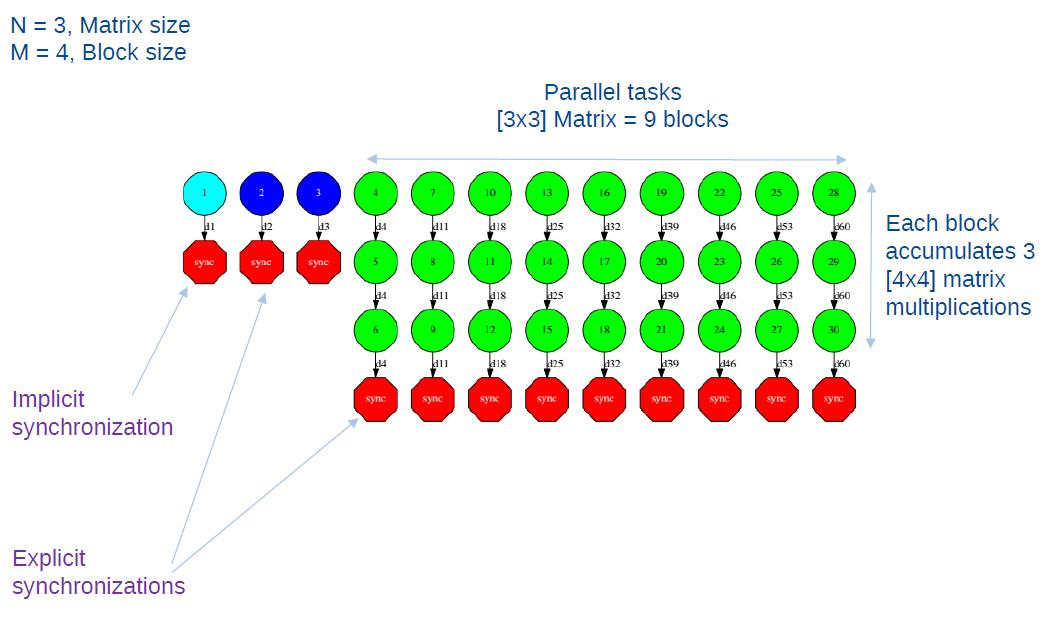
\includegraphics[width=1.0\textwidth]{./Sections/6_Bindings/Figures/matmul.jpeg}
    %\caption{Matmul Execution Graph.}
    %\label{fig:BLAST_workflow}
\end{figure}

\subsection{Python}

COMPSs features a binding for Python 2.x applications. The next subsections explain how to program a Python 
application for COMPSs and how to configure the binding library.

\subsubsection{Programming Model}

\paragraph{Task Selection}

Like in the case of the Java language, a COMPSs Python application is a sequential program that contains calls 
to tasks. In particular, the user can select as a task:

\begin{itemize}
 \item Functions
 \item Instance methods: methods invoked on objects.
 \item Class methods: static methods belonging to a class.
\end{itemize}

Regarding task selection, in Python it is not done by means of an annotated interface but with the use of 
Python decorators. In particular, the user needs to add, before the definition of the function/method, 
a @task decorator that describes the task.

As an example, let us assume that the application calls a function func, which receives a string parameter 
containing a file name and an integer parameter. The code of func updates the file.

\begin{lstlisting}[language=python]
my_file = 'sample_file.txt'
func(my_file, 1)
\end{lstlisting}

In order to select {\it func} as a task, the corresponding {\it @task} decorator needs to be placed right 
before the definition of the function, providing some metadata about the parameters of that function. 
The metadata corresponding to a parameter is specified as an argument of the decorator, whose name is 
the formal parameter’s name and whose value defines the type and direction of the parameter. 
The parameter types and directions can be:

\begin{itemize}
 \item Types: {\it primitive types} (integer, long, float, boolean), {\it strings}, {\it objects} (instances of user-defined classes, dictionaries, lists, tuples, complex numbers) and {\it files} are supported.
 \item Direction: it can be read-only ({\it IN} - default), read-write ({\it INOUT}) or write-only ({\it OUT}).
\end{itemize}

COMPSs is able to automatically infer the parameter type for primitive types, strings and objects, 
while the user needs to specify it for files. On the other hand, the direction is only mandatory for 
{\it INOUT} and {\it OUT} parameters. Thus, when defining the parameter metadata in the {\it @task} 
decorator, the user has the following options:

\begin{itemize}
 \item {\it INOUT}: the parameter is read-write. The type will be inferred.
 \item {\it OUT}: the parameter is write-only. The type will be inferred.
 \item {\it FILE}: the parameter is a file. The direction is assumed to be {\it IN}.
 \item {\it FILE\_INOUT}: the parameter is a read-write file.
 \item {\it FILE\_OUT}: the parameter is a write-only file.
\end{itemize}
     
Consequently, please note that in the following cases there is no need to include an argument in 
the {\it @task} decorator for a given task parameter:

\begin{itemize}
 \item Parameters of primitive types (integer, long, float, boolean) and strings: the type of these 
       parameters can be automatically inferred by COMPSs, and their direction is always {\it IN}.
 \item Read-only object parameters: the type of the parameter is automatically inferred, and the 
       direction defaults to {\it IN}.
\end{itemize}
 
Continuing with the example, in the following code snippet the decorator specifies that {\it func} 
has a parameter called {\it fi}, of type {\it FILE} and {\it INOUT} direction. Note how the second 
parameter, {\it i}, does not need to be specified, since its type (integer) and direction ({\it IN}) 
are automatically inferred by COMPSs.

\begin{lstlisting}[language=python]
from pycompss.api.task import task
from pycompss.api.parameter import *
%*{\bf @task }*)(f = FILE_INOUT)
def func(f, i):
     fd = open(f, ‘r+’)
     ...
\end{lstlisting}

If the function or method returns a value, the programmer must specify the type of that value using 
the {\it returns} argument of the {\it @task} decorator:

\begin{lstlisting}[language=python]
@task(%*{\bf returns }*) = int)
def ret_func():
     return 1
\end{lstlisting}

For tasks corresponding to instance methods, by default the task is assumed to modify the callee object 
(the object on which the method is invoked). The programmer can tell otherwise by setting the 
{\it isModifier} argument of the {\it @task} decorator to {\it False}.

\begin{lstlisting}[language=python]
class MyClass(object):
    ...
    @task(%*{\bf isModifier }*) = False)
    def instance_method(self):
        ... # self is NOT modified here
\end{lstlisting}

The programmer can also mark a task as a high-priority task with the {\it priority} argument of the 
{\it @task} decorator. This way, when the task is free of dependencies, it will be scheduled before 
any of the available low-priority (regular) tasks. This functionality is useful for tasks that are in 
the critical path of the application’s task dependency graph.

\begin{lstlisting}[language=python]
@task(%*{\bf priority }*) = True)
def func():
    ...
\end{lstlisting}

Table \ref{tab:task_decorator_arguments} summarizes the arguments that can be found in the @task decorator.

\begin{longtable}{| p{0.31\textwidth} | p{0.69\textwidth} |}
\hline
\multicolumn{1}{|c|}{{\bf Argument }}    &  \multicolumn{1}{c|}{{\bf Value }}\\
\hline
\multirow{5}{*}{Formal parameter name}  &  - INOUT: read-write parameter, all types except file (primitives, strings, objects). \\
& - OUT: read-write parameter, all types except file (primitives, strings, objects). \\
& - FILE: read-only file parameter. \\
& - FILE\_INOUT: read-write file parameter. \\
& - FILE\_OUT: write-only file parameter. \\
\hline
returns & int (for integer and boolean), long, float, str, dict, list, tuple, user-defined classes \\
\hline
isModifier &  True (default) or False \\
\hline
priority  & True or False (default) \\
\hline
\caption{Arguments of the {\it @task} decorator.}
\label{tab:task_decorator_arguments}
\end{longtable}


\paragraph{Main Program}
The main program of the application is a sequential code that contains calls to the selected tasks. 
In addition, when synchronizing for task data from the main program, 
there exist two API functions that need to be invoked:

\begin{itemize}
 \item {\it compss\_open(file\_name, mode = 'r')}: similar to the Python {\it open()} call. It synchronizes
       for the last version of file {\it file\_name} and returns the file descriptor for that synchronized
       file. It can receive an optional parameter {\it mode}, which defaults to '{\it r}', containing the
       mode in which the file will be opened (the open modes are analogous to those of
       Python {\it open()}).
 \item {\it compss\_wait\_on(obj, to\_write = True)}: synchronizes for the last version of object {\it obj}
       and returns the synchronized object. It can receive an optional boolean parameter
       {\it to\_write}, which defaults to {\it True}, that indicates whether the main program will modify the
       returned object.
\end{itemize}

To illustrate the use of the aforementioned API functions, the following example first invokes a task 
{\it func} that writes a file, which is later synchronized by calling {\it compss\_open()}. 
Later in the program, an object of class {\it MyClass} is created and a task method {\it method} 
that modifies the object is invoked on it; the object is then synchronized with {\it compss\_wait\_on()}, 
so that it can be used in the main program from that point on.

\begin{lstlisting}[language=python]
from pycompss.api.api import compss_open, compss_wait_on

my_file = 'file.txt'
func(my_file)
fd = %*{\bf compss\_open}*)(my_file)
...

my_obj = MyClass()
my_obj.method()
my_obj = %*{\bf compss\_wait\_on}*)(my_obj)
...
\end{lstlisting}

The corresponding task selection for the example above would be:

\begin{lstlisting}[language=python]
@task(f = FILE_OUT)
def func(f):
    ...
    
    class MyClass(object):
        ...
        
        @task()
        def method(self):
            ... # self is modified here
\end{lstlisting}

Table \ref{tab:python_api_functions} summarizes the API functions to be used in the main program of a COMPSs Python application.

\begin{longtable}{| p{0.30\textwidth} | p{0.7\textwidth} |}
\hline
\multicolumn{1}{|c|}{{\bf Function }}    &  \multicolumn{1}{c|}{{\bf Use }}\\
\hline
compss\_open(file\_name, mode = 'r') & Synchronizes for the last version of a file and returns its file descriptor. \\
\hline
compss\_wait\_on(obj, to\_write = True) & Synchronizes for the last version of an object and returns it. \\
\hline
\caption{COMPSs Python API functions.}
\label{tab:python_api_functions}
\end{longtable}


\subparagraph{Future Objects}
If the programmer selects as a task a function or method that returns a value, that value is not 
generated until the task executes. However, in order to keep the asynchrony of the task invocation, 
COMPSs manages future objects: a representant object is immediately returned to the main program when 
a task is invoked.

\begin{lstlisting}[language=python]
@task(%*{\bf returns }*) = MyClass)
def ret_func():
    return MyClass(...)

...

# %*{\bf o }*) is a future object
o = ret_func()
\end{lstlisting}

The future object returned can be involved in a subsequent task call, and the COMPSs runtime will automatically 
find the corresponding data dependency. In the following example, the future object o is passed as a parameter 
and callee of two subsequent (asynchronous) tasks, respectively:

\begin{lstlisting}[language=python]
# %*{\bf o }*) is a future object
o = ret_func()

...

another_task(o)

...

o.yet_another_task()
\end{lstlisting}

In order to synchronize the future object from the main program, the programmer proceeds in the same way 
as with any object updated by a task:

\begin{lstlisting}[language=python]
# %*{\bf o }*) is a future object
o = ret_func()

...

o = compss_wait_on(o)
\end{lstlisting}
                         
The future object mechanism is applied to primitive types, strings and objects (including the Python 
built-in types list, dictionary and tuple).

It is important to note that, for instances of user-defined classes, the classes of these objects 
should have an empty constructor, otherwise the programmer will not be able to invoke task instance 
methods on those objects:
                                   
\begin{lstlisting}[language=python]
class MyClass(object):
    def __init__(self): # empty constructor
        ...
        
    ...

o = ret_func()

# invoking a task instance method on a future object can only
# be done when an empty constructor is defined in the object's
# class
o.yet_another_task()
\end{lstlisting}

\paragraph{Important Notes}
For the COMPSs Python binding to function correctly, the programmer should not use relative imports 
in her code. Relative imports can lead to ambiguous code and they are discouraged in Python, as explained in:

\begin{lstlisting}[language=html]
http://docs.python.org/2/faq/programming.html#what-are-the-best-practices-for-using-import-in-a-module
\end{lstlisting}

\subsubsection{Application Execution}
The next subsections describe how to execute applications with the COMPSs Python binding.

\paragraph{Environment}
The following environment variables must be defined before executing a COMPSs Python application:

JAVA\_HOME: Java JDK installation directory (e.g. /usr/lib/jvm/java-6-openjdk/)

\paragraph{Command}

In order to run a Python application with COMPSs, the script runcompssext can be used, like for 
Java and C/C++ applications. An example of an invocation of the script is:

\begin{lstlisting}[language=bash]
> runcompssext
  --lang=python
  --app=$TEST_DIR/test.py
  --classpath=$TEST_DIR
  --library_path=/home/user/libdir
  --cline_args="arg1 arg2"
  --project=$TEST_DIR/project.xml
  --resources=$TEST_DIR/resources.xml
  --tracing=true
\end{lstlisting}

The options of the script are:

\begin{lstlisting}[language=bash]
  --lang=python
  --app=<path>: path to the .py file containing the main program.
  --classpath=<path>: path/s where to search for the application’s Python modules. The default value is the current directory.
  --library_path=<path>: path/s where to search for libraries that are not in a standard path. The default value is the variable $LD_LIBRARY_PATH.
  --cline_args=<args>: arguments to pass to the application.
  --project=<proj_file>: path of the project XML file.
  --resources=<res_file>: path of the resources XML file.
  --tracing=<true | false>: generate execution traces. Default is false.
\end{lstlisting}
           
  \section{Tracing}
\label{sec:Tracing}

COMPSs runtime can generate a post-execution trace of the distributed execution of the application. 
This trace is useful for performance analysis and diagnosis.

A trace file may contain different events as task-execution or file-transfer events among others. 
(In the current release we only support task-execution events and we intend to support file-transfer evens in a future release).

During the execution of the application, an XML file is created at worker nodes to keep track of 
these events. At the end of the execution, all the XML files are merged to get a final trace file.

In the following sections we will explain the command used for tracing, how the events are registered, 
in a process called instrumentation, how to visualize the trace file and make a good analysis of 
performance based on the data shown in the trace.

\subsection{Trace Command}
In order to obtain a post-execution trace file the option ``{\bf --tracing}'' of the 
``{\bf runcompssext}'' command script must be set to ``{\bf true}''. This command is available in 
the system path after COMPSs runtime installation.

Here is the example of the command execution with the tracing option enabled for our Hmmer application.

\begin{lstlisting}[language=bash]
runcompssext --app=hmmerobj.HMMPfam --tracing=true --cline_args="/sharedDisk/Hmmer/smart.HMMs.bin /sharedDisk/Hmmer/256seq   /home/user/out.txt 2 8 -A 222"
\end{lstlisting}
 

\subsection{Application Instrumentation}

The instrumentation is the process that intercepts different events of the application execution 
and keeps log of them. This will cause an overhead in the execution time of the application that 
the user should take into account, but the collected data will be extremely useful for performance 
analysis and diagnosis.

COMPSs runtime uses the Extrae tool from BSC to dynamically instrument the application. 
At worker nodes, in background, Extrae keeps track of the events in an intermediate format 
file (with .mpit extension). In the master, at the end of the execution, Extrae merges the 
intermediate files to get the final trace file, a Paraver format file (.prv). See the visualization 
section in this manual for the Paraver tool.

When instrumenting the application Extrae will output several messages before and after the whole 
user application execution, at the master, and before and after a task execution, at the workers. 
No messages are output during the execution.

\begin{lstlisting}[language=bash]
------------- Executing hmmerobj.HMMPfam ------------------

[   API]  -  Deploying the Integrated Toolkit
[   API]  -  Starting the Integrated Toolkit
[   API]  -  Initializing components

Welcome to Extrae 2.4.3rc4 (revision 311 based on framework/trunk/files/extrae)
Extrae: Generating intermediate files for Paraver traces.
Extrae: Intermediate files will be stored in /home/user/IT/hmmerobj.HMMPfam
Extrae: Tracing buffer can hold 500000 events
Extrae: Tracing mode is set to: Detail.
Extrae: Successfully initiated with 1 tasks

[   API]  -  Ready to process tasks

...
...
...
[   API]  -  No more tasks for app 1
[   API]  -  Stopping IT
[   API]  -  Cleaning

Extrae: Application has ended. Tracing has been terminated.
...

merger: Output trace format is: Paraver
merger: Extrae 2.4.3rc4 (revision 311 based on framework/trunk/files/extrae)
...

[   API]  -  Integrated Toolkit stopped
...

mpi2prv: Selected output trace format is Paraver

mpi2prv: Parsing intermediate files

mpi2prv: Generating tracefile (intermediate buffers of 1342156 events)

mpi2prv: Congratulations! hmmerobj.HMMPfam_compss_trace_1392736225.prv has been generated.

------------------------------------------------------------
\end{lstlisting}

For more information about Extrae please visit the following site: 
\begin{center}
\url{http://www.bsc.es/computer-science/extrae} 
\end{center}


\subsection{Trace Visualization}

Paraver is the BSC tool for trace visualization. Trace events are encoded in Paraver (.prv) 
format by the Extrae tool (see previous section). Paraver is a powerful tool, it can show many 
views of the trace data by mean of different configuration files, and the user can load and 
modify these configuration files or create new ones.

In the following subsections we will see how to load a trace file into Paraver, open the task 
events view by mean of an already predefined configuration file that is provided, and how to 
adjust the view to display the data in the proper way.

For more information about Paraver please visit the following site:

\begin{center}
\url{http://www.bsc.es/computer-sciences/performance-tools/paraver}
\end{center}

\subsubsection{Trace Loading}

The final trace file in Paraver format (.prv) can be found at the application directory under 
the IT directory after the traced-application execution ends. The fastest way to open it is 
calling directly the Paraver command passing to it the trace filename as argument.

\begin{lstlisting}[language=bash]
wxparaver /home/user/IT/hmmerobj.HMMPfam/*.prv
\end{lstlisting}
 
\subsubsection{Configuration File}
In order to open a view with the task events of the application, an already predefined configuration 
file is provided. To open it, just go in the main window to the ``Load Configuration'' option in 
the menu ``File''. The configuration file is under the following path ``/opt/COMPSs/paraver/cfgs/tasks.cfg''. 
After accepting the load of the configuration file, another window will appear to show the view.

\begin{figure}[ht!]
  \centering
    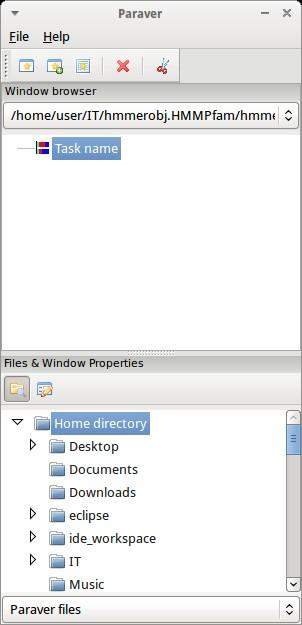
\includegraphics[width=0.45\textwidth]{./Sections/7_Tracing/Figures/1.jpeg}
    %\caption{Caption.}
    %\label{fig:matrix}
\end{figure}

\begin{figure}[ht!]
  \centering
    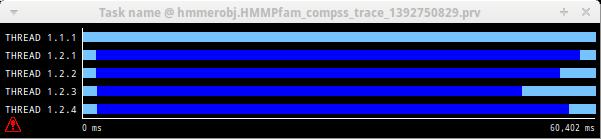
\includegraphics[width=1.0\textwidth]{./Sections/7_Tracing/Figures/2.jpeg}
    %\caption{Caption.}
    %\label{fig:matrix}
\end{figure}

\subsubsection{View Adjustment}
In a Paraver view, a red exclamation sign may appear on the bottom-left corner (see last picture in 
previous section). This means that some little adjustments must be done to view the trace correctly:

\begin{itemize}
 \item Fit window: this will give a better color scale to identify events.
 \begin{itemize}
  \item Right click on the trace window
  \item Chose the option Fit Semantic Scale / Fit Both
 \end{itemize}
\end{itemize}

\begin{figure}[ht!]
  \centering
    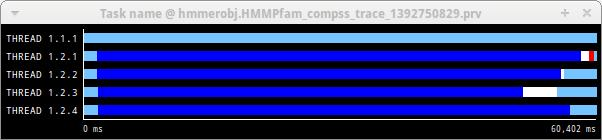
\includegraphics[width=1.0\textwidth]{./Sections/7_Tracing/Figures/3.jpeg}
    %\caption{Caption.}
    %\label{fig:matrix}
\end{figure}

\begin{itemize} 
 \item View Event Flags: This will put a flag whenever an event starts/ends.
\begin{itemize}
 \item Right click on the trace window
 \item Chose the option View / Event Flags
\end{itemize}
\end{itemize}
 
\begin{figure}[ht!]
  \centering
    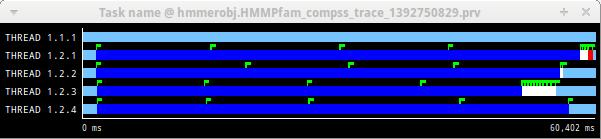
\includegraphics[width=1.0\textwidth]{./Sections/7_Tracing/Figures/4.jpeg}
    %\caption{Caption.}
    %\label{fig:matrix}
\end{figure}

\begin{itemize}
 \item Show Info Panel: This will show an information panel. In the tab ``Colors'' we can see the legend of the colors shown in the view.
 \begin{itemize}
  \item Right click on the trace window
  \item Check the Info Panel option
  \item Select the Colors tab in the panel
 \end{itemize}
\end{itemize}

\begin{figure}[ht!]
  \centering
    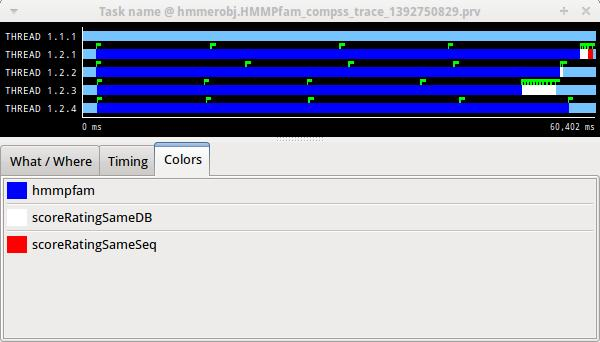
\includegraphics[width=1.0\textwidth]{./Sections/7_Tracing/Figures/5.jpeg}
    %\caption{Caption.}
    %\label{fig:matrix}
\end{figure}

\begin{itemize}
 \item Zoom: In order to understand a trace view better, sometimes it’s a worth thing to zoom into it a little.
 \begin{itemize}
  \item Select a region in the trace window to see that region in detail
  \item And repeat the previous step as many times as needed
  \item The undo-zoom option is in the right click panel
 \end{itemize}
\end{itemize}

\begin{figure}[ht!]
  \centering
    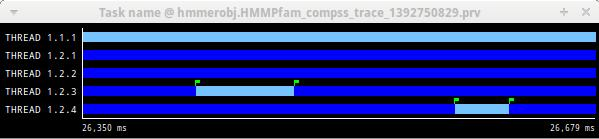
\includegraphics[width=1.0\textwidth]{./Sections/7_Tracing/Figures/6.jpeg}
    %\caption{Caption.}
    %\label{fig:matrix}
\end{figure}

\begin{figure}[ht!]
  \centering
    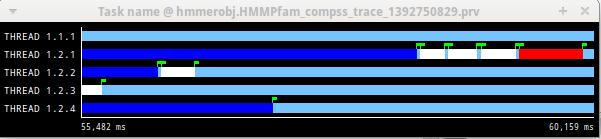
\includegraphics[width=1.0\textwidth]{./Sections/7_Tracing/Figures/6_2.jpeg}
    %\caption{Caption.}
    %\label{fig:matrix}
\end{figure}


\subsection{Trace Interpretation}
In this section we will explain how to interpret a trace view once it has been adjusted as 
described in the previous section.

\begin{itemize}
 \item The trace view has in its horizontal axis the execution time and in the vertical 
       axis one line for the master at the top, and below it, one line for each of the workers.
 \item In a line, the light blue color means idle state, in the sense that there is no event at that time.
 \item Whenever an event starts or ends a flag is shown.
 \item In the middle of an event, the line shows a different color. Colors are assigned depending on the event type.
 \item In the info panel the legend of assigned color to event type is provided.
\end{itemize}

\begin{figure}[ht!]
  \centering
    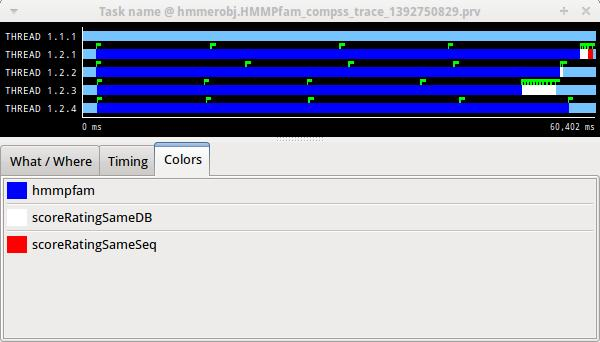
\includegraphics[width=1.0\textwidth]{./Sections/7_Tracing/Figures/7.jpeg}
    %\caption{Caption.}
    %\label{fig:matrix}
\end{figure}

\subsection{Trace Analysis}

In this section, we will give some tips to analyse a COMPSs trace from two points of view 
graphical and numerical.

\subsubsection{Graphical Analysis}

The main concept is that computational events, the task events in this case, must be well 
distributed among all workers to have a good parallelism, and the duration of task events 
should be also balanced, this means, the duration of computational bursts.

\begin{figure}[ht!]
  \centering
    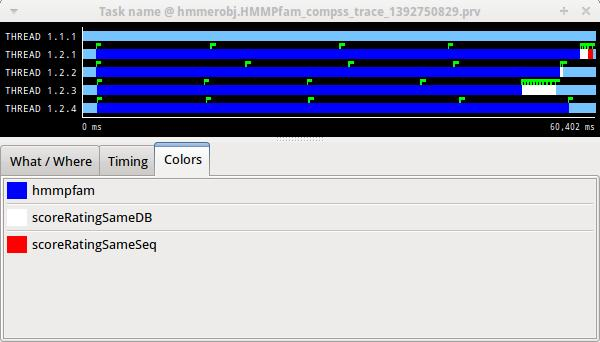
\includegraphics[width=1.0\textwidth]{./Sections/7_Tracing/Figures/8.jpeg}
    %\caption{Caption.}
    %\label{fig:matrix}
\end{figure}

In the previous trace view, all the tasks of type ``hmmpfam'' in dark blue appear to be well 
distributed among the four workers, each worker executes four ``hmmpfam'' tasks.

But some workers finish earlier than the others, worker 1.2.3 finish the first and worker 1.2.1 
the last. So there is an imbalance in the duration of ``hmmpfam'' tasks. The programmer should 
analyse then whether all the tasks process the same amount of input data and do the same thing 
in order to find out the reason of such imbalance.

Another thing to highlight is that tasks of type ``scoreRatingSameDB'' are not equal distributed 
among all the workers. There are workers that execute more tasks of this type than the others. 
To understand better what happens here, let’s take a look to the execution graph and also zoom 
in the last part of the trace.

\begin{figure}[ht!]
  \centering
    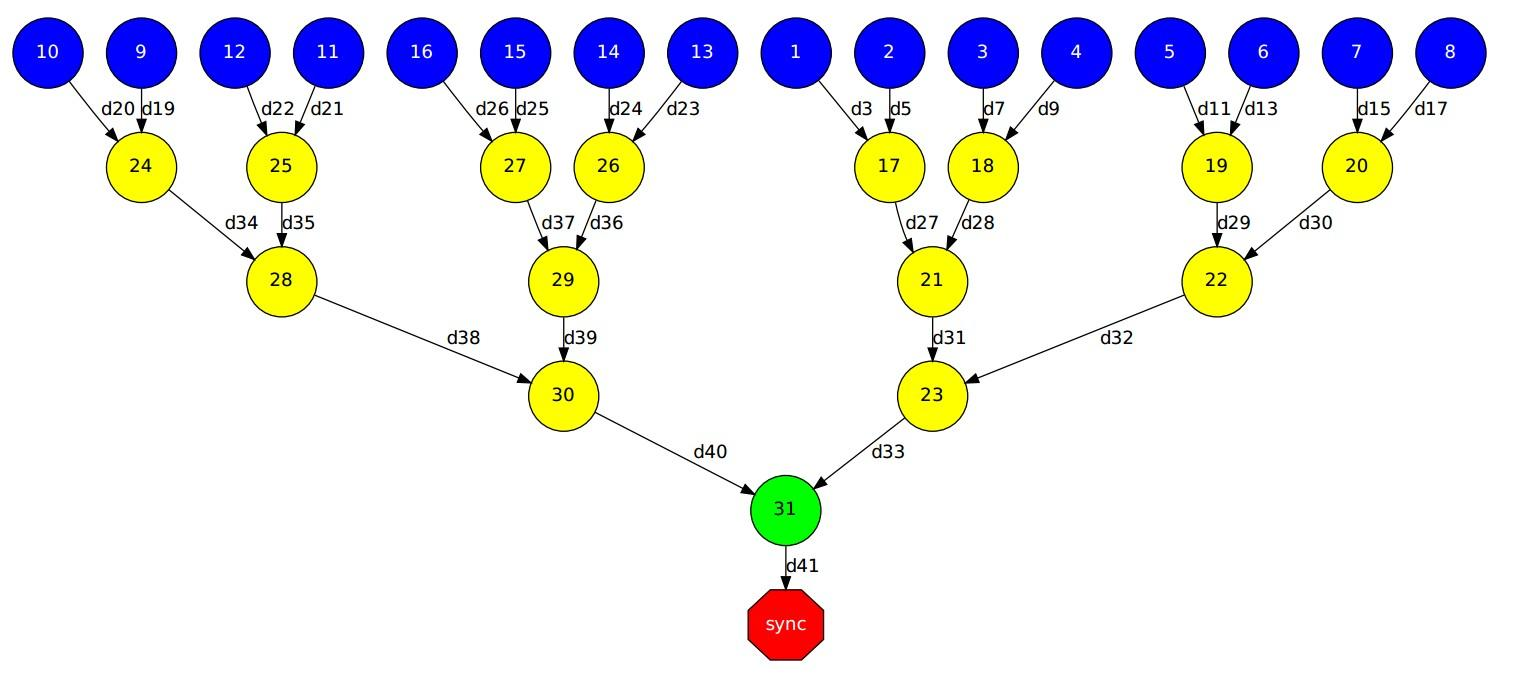
\includegraphics[width=1.0\textwidth]{./Sections/7_Tracing/Figures/9.jpeg}
    %\caption{Caption.}
    %\label{fig:matrix}
\end{figure}

\begin{figure}[ht!]
  \centering
    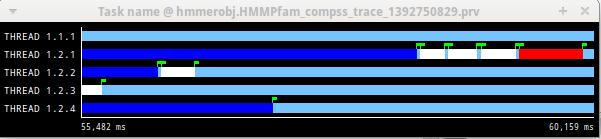
\includegraphics[width=1.0\textwidth]{./Sections/7_Tracing/Figures/10.jpeg}
    %\caption{Caption.}
    %\label{fig:matrix}
\end{figure}


There is only one task of type ``scoreRatingSameSeq''. This task appears in red in the trace 
(and in light-green in the graph). With the help of the graph we see that the ``scoreRatingSameSeq'' 
task has dependences on tasks of type ``scoreRatingSameDB'', in white (or yellow).

When the last task of type ``hmmpfam'' (in dark blue) ends, the last dependences are solved, 
and if we look at the graph, this means going across a path of three dependences of type 
``scoreRatingSameDB'' (in yellow). And because of these are sequential dependences (one depends 
on the previous) no more than a worker can be used at the same time to execute the tasks. 
This is the reason of why the last three task of type ``scoreRatingSameDB'' (in white) are 
executed in worker 1.2.1 sequentially.

\subsubsection{Numerical Analysis}
Here we show another trace from a different parallel execution of the Hmmer program.
 
\begin{figure}[ht!]
  \centering
    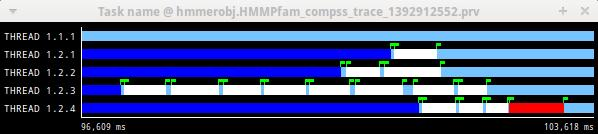
\includegraphics[width=1.0\textwidth]{./Sections/7_Tracing/Figures/11.jpeg}
    %\caption{Caption.}
    %\label{fig:matrix}
\end{figure} 
 
Paraver offers the possibility of having different histograms of the trace events. 
For it just click the ``New Histogram'' button in the main window and accept the 
default options in the ``New Histogram'' window that will appear.

\begin{figure}[ht!]
  \centering
    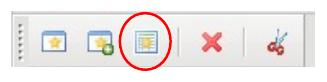
\includegraphics[width=0.5\textwidth]{./Sections/7_Tracing/Figures/12.jpeg}
    %\caption{Caption.}
    %\label{fig:matrix}
\end{figure}

After that, the following table is shown. In this case for each worker, the time spent 
executing each type of task is shown. Task names appear in the same color than in the 
trace view. The color of a cell in a row corresponding to a worker goes in a scale from 
a light-green for lower values to a dark-blue for higher ones. This conforms a color based histogram.

\begin{figure}[ht!]
  \centering
    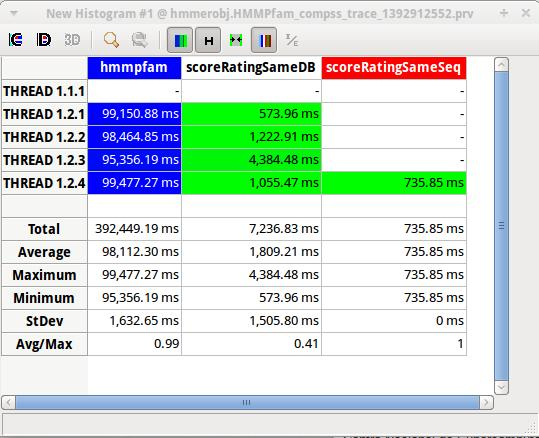
\includegraphics[width=0.8\textwidth]{./Sections/7_Tracing/Figures/13.jpeg}
    %\caption{Caption.}
    %\label{fig:matrix}
\end{figure}
 
The previous table also gives, at the end of each column, some extra statistical 
information for each type of tasks (as the total, average, maximum or minimum values, etc.).

In the window properties of the main window we can change the semantic of the statistics 
to see other factors rather than the time, for example, the number of burst.

\begin{figure}[ht!]
  \centering
    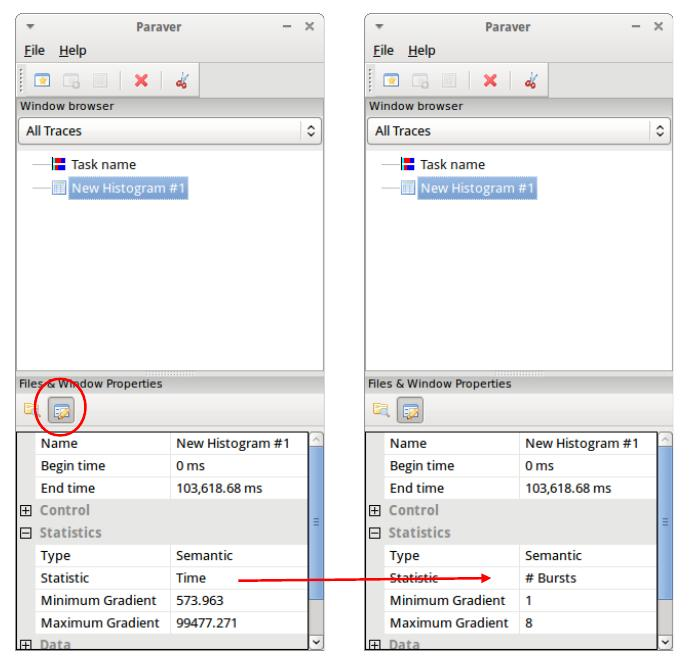
\includegraphics[width=0.8\textwidth]{./Sections/7_Tracing/Figures/14.jpeg}
    %\caption{Caption.}
    %\label{fig:matrix}
\end{figure}

In the same way as before, the following table shows for each worker the number of bursts 
for each type of task, this is, the number or tasks executed of each type. Notice the gradient 
scale from light-green to dark-blue changes with the new values.

\begin{figure}[ht!]
  \centering
    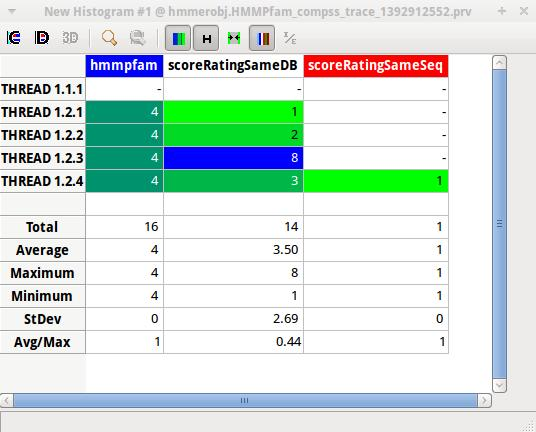
\includegraphics[width=0.8\textwidth]{./Sections/7_Tracing/Figures/15.jpeg}
    %\caption{Caption.}
    %\label{fig:matrix}
\end{figure}

\subsubsection{Other Trace examples}

To end this section, let’s present some other examples of COMPSs traces. COMPSs traces can be 
much complex as the number of workers or tasks grows. Just to illustrate this, the following 
pictures show traces with a greater number of workers and tasks.

\begin{figure}[ht!]
  \centering
    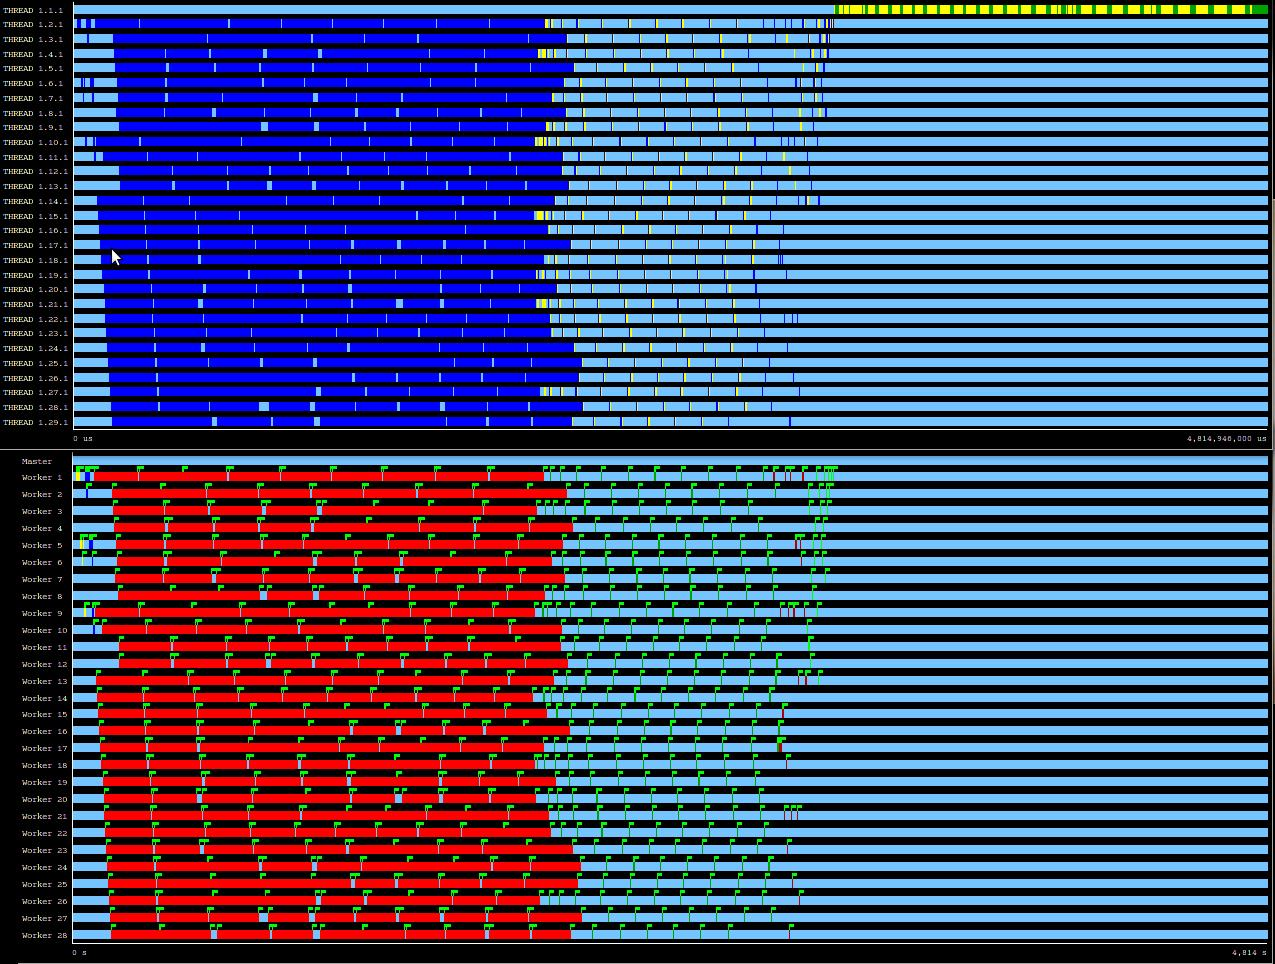
\includegraphics[width=0.91\textwidth]{./Sections/7_Tracing/Figures/16.jpeg}
    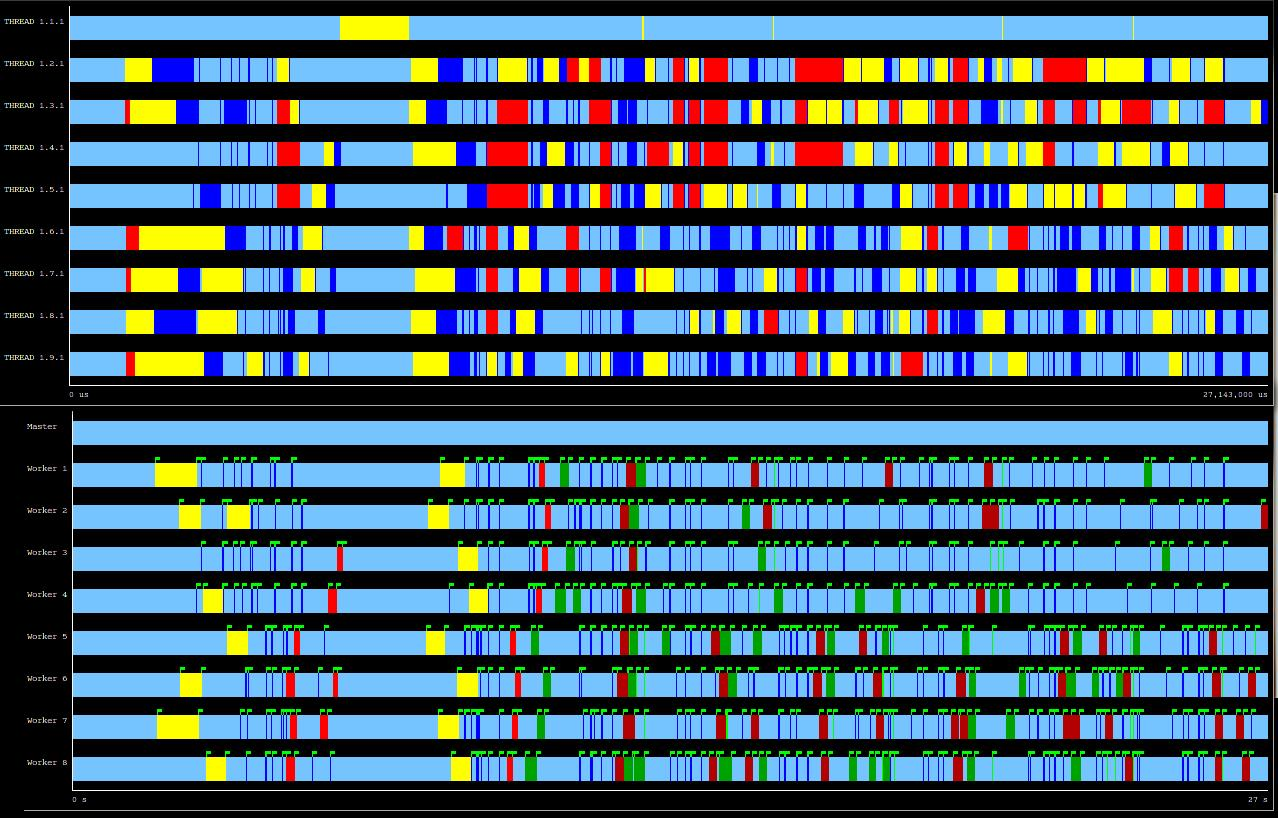
\includegraphics[width=0.91\textwidth]{./Sections/7_Tracing/Figures/16_2.jpeg}
    %\caption{Caption.}
    %\label{fig:matrix}
\end{figure}


  
  %%%%%%%% END PAGE %%%%%%%%%

  \newpage

  \vspace*{\fill} 
  \begin{center}
  Please find more details on the COMPSs framework at

  \Huge{\url{www.bsc.es/compss}}
  \end{center}    
  \vspace*{\fill} 
           
        
\end{document}
